\documentclass[12pt]{mwart}

\usepackage{polski}
\usepackage[utf8]{inputenc}
\usepackage{mathtools,amsthm,amssymb,icomma,upgreek,xfrac,graphics,scrextend,float,tabularx,hyperref,multicol,array,caption,enumitem}
\usepackage[table,xcdraw]{xcolor}

\mathtoolsset{mathic}
\raggedbottom
\graphicspath{ {./images/} }
\renewcommand{\refname}{Źródła}
\captionsetup{justification=raggedright,singlelinecheck=true}

\newcommand{\indep}{\perp \!\!\! \perp}
\begin{document}
	
	\begin{center}
		{\Large\textbf{Symulacje komputerowe}}
	\end{center}
	\begin{center}
		Raport 2
	\end{center}
	
	\noindent Temat: \ \textbf{Proces Ryzyka i ruch Browna}\\
	Imię i Nazwisko prowadzącego kurs: \ \textbf{Dr Michał Balcerek}	\newline\newline
	
	
	\noindent\begin{tabularx}{\textwidth}{|X |X|}
		\hline
		\begin{center}
			Imię i Nazwisko,\\ nr indeksu
		\end{center} &  \begin{center}
			Kacper Brudnik, 262286\\
			Szymon Malec, 262276
		\end{center}\\\hline
		Wydział: & Wydział matematyki, W13 \\\hline
		Dzień i godzina zajęć: & Wtorek,\vphantom{ $11^{1^{5}}$} $11^{15}$\\\hline
		Kod grupy ćwiczeniowej: & T00-70d \\\hline
		Data oddania raportu: & 26.06.2022 \\\hline
		\textbf{Ocena końcowa} &\\\hline
	\end{tabularx}\newline\newline
	
	\noindent\textbf{Adnotacje i uwagi:}
	
	\newpage
	
	
	\section{Wstęp}
	\noindent Drugi raport z symulacji komputerowych został podzielony na dwa zadania. Celem pierwszego z nich było dopasowanie modelu Ryzyka do otrzymanych danych oraz oszacowanie prawdopodobieństwa ruiny w skończonym i nieskończonym czasie. W tym celu:
	\begin{itemize}[leftmargin=10mm, label=\small$\bullet$]
		\item Znaleźliśmy rozkład zmiennej losowej $X_i$ oznaczającej wielkość $i$-tej szkody.
		\item Wyestymowaliśmy pozostałe parametry procesu:
		\begin{enumerate}[leftmargin=10mm]
			\item $\lambda$ -- intensywność jednorodnego procesu Poissona;
			\item $\theta$ -- parametr odpowiedzialny za wysokość premii.
		\end{enumerate}
		\item Oszacowaliśmy prawdopodobieństwo ruiny dla czasu:
		\begin{enumerate}[leftmargin=10mm]
			\item skończonego przy pomocy metody Monte Carlo,
			\item nieskończonego przy pomocy algorytmu Pollaczka-Chinczyna.
		\end{enumerate}
	\end{itemize}
	\noindent Drugie zadanie polegało natomiast na oszacowaniu średniego czasu wyjścia ruchu Browna z zadanego przedziału w zależności od punktu startowego. Dodatkowo mieliśmy oszacować prawdopodobieństwo wyjścia przez dany koniec odcinka. Pokazaliśmy, że wybór przedziału może być dowolny i łatwo go uogólnić na dowolny inny przedział. Na koniec, przy pomocy pakietów matematycznych, dopasowaliśmy funkcję do wygenerowanych metodą Monte Carlo danych.
	
	
	
	\section{Zadanie 1}

	\subsection{Jednorodny proces Poissona}
	
	\noindent Jednorodnym procesem Poissona z intensywnością $\lambda > 0$ nazywamy proces liczący $\{N_t\}_{t \geq 0}$, który spełnia:
	\begin{itemize}[leftmargin=10mm, label={\small$\bullet$}]
		\item $N_0 = 0$,
		\item $N_t$ ma niezależne przyrosty,
		\item $N_t$ ma stacjonarne przyrosty,
		\item $N_t \sim \mathcal{P}oiss(\lambda t)$.
	\end{itemize}
	Proces ten służy do zliczania wystąpień pewnych zdarzeń losowych, których częstość występowania (intensywność) jest cały czas taka sama.\\
	
	\noindent Do symulacji procesu Poissona przydaje się jedna z jego własności, którą jest to, że odstępy czasowe pomiędzy skokami mają rozkład $\mathcal{E}xp(\lambda)$.
	Oznacza to, że jeśli chcemy wygenerować jedną trajektorię na przedziale $[0, T]$, to wystarczy generować kolejne $X_i \sim \mathcal{E}xp(\lambda)$, aż ich suma przekroczy $T$.\\
	
	\noindent \textbf{Algorytm}
	\begin{enumerate}[leftmargin=10mm]
		\item Definiuj $I = 0$, $t=0$.
		\item Generuj $X \sim \mathcal{E}xp(\lambda)$.
		\item $t = t + X$. Jeśli $t > T$, przerwij i zwróć $\{S_i\}$. W przeciwnym razie $I = I + 1$, $S_I = t$.
		\item Wróć do kroku 2.
	\end{enumerate}
	Otrzymane z powyższego algorytmu $\{S_i\}$ to czasy oczekiwania na i-ty skok od startu trajektorii.
	
	\begin{figure}[H]
		\centering
		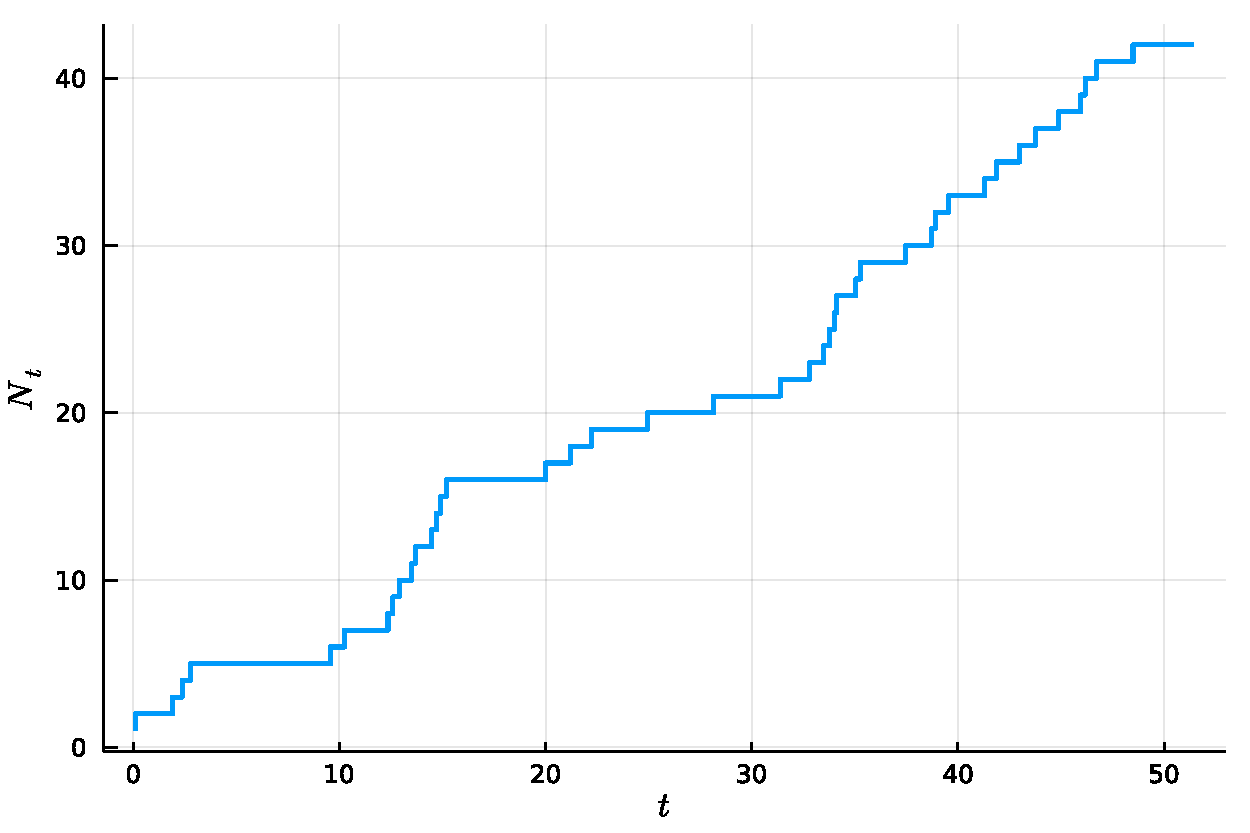
\includegraphics[width=\columnwidth]{fig/poisson.pdf}
		\caption{Przykładowa trajektoria procesu Poisson z intensywnością $\lambda = 1$.}
	\end{figure}
	
	
	
	\subsection{Klasyczny proces Ryzyka}
	
	\noindent Klasycznym procesem Ryzyka nazywamy proces stochastyczny opisujący kapitał firmy ubezpieczeniowej postaci
	$$ R_t = u + ct - \sum_{i=1}^{N_t} X_i, $$
	gdzie
	\begin{itemize}[leftmargin=10mm, label={\small$\bullet$}]
		\item $u > 0$ -- kapitał początkowy,
		\item $ct$ -- stałe przychody ($c > 0$),
		\item $N_t$ -- jednorodny proces Poissona z intensywnością $\lambda > 0$,
		\item $X_i$ -- ciąg niezależnych zmiennych losowych o tym samym rozkładzie opisujący straty, $\mathbb{E}X_i = \mu$, $X_i > 0$.
	\end{itemize}
	Proces ten odgrywa ważną rolę w branży ubezpieczeniowej, ponieważ symulacja tego procesu pozwala oszacować prawdopodobieństwo bankructwa firmy oraz jej średni zysk. Dzięki temu jesteśmy w stanie określić jaka powinna być cena ubezpieczenia, by takie prawdopodobieństwo nie było zbyt wysokie, a zysk zadowalający.\vspace{1.5mm}\\
	Parametrem odpowiadającym za przychody jest stała $c$. Do odpowiedniego doboru tego parametru wykorzystuje się wzór
	\begin{equation}\label{c}
		c = (1 + \theta)\mu\lambda
	\end{equation}
	gdzie $\theta > 0$ jest parametrem odpowiadającym za wysokość premii.\\
	
	\noindent \textbf{Algorytm}
	\begin{enumerate}[leftmargin=10mm]
		\item Generuj $N_t$ na przedziale $[0, T]$.
		\item Generuj $X_1, \dots, X_{N_t}$.
		\item Zwróć $R_t = u + ct - \sum\limits_{i=1}^{N_t} X_i$.
	\end{enumerate}
	
	
	
	\subsection{Dopasowanie modelu do danych}
	
	\noindent Zastosujemy teraz proces Ryzyka w praktyce. Postaramy się jak najlepiej dopasować model klasycznego procesu Ryzyka do danych, które zostały nam udostępnione przez prowadzącego zajęcia laboratoryjne. Dane te opisują 50 trajektorii pewnego klasycznego procesu Ryzyka. Naszym celem jest wyznaczenie parametrów tego procesu na podstawie danych, by móc następnie przeprowadzać jego symulacje.\vspace{1.5mm}\\
	Badany proces został wysymulowany na odcinku $[0, 100]$ z krokiem czasowym $h = 0,01$. Kapitał początkowy wynosi $u = 50$.
	
	\begin{figure}[H]
		\centering
		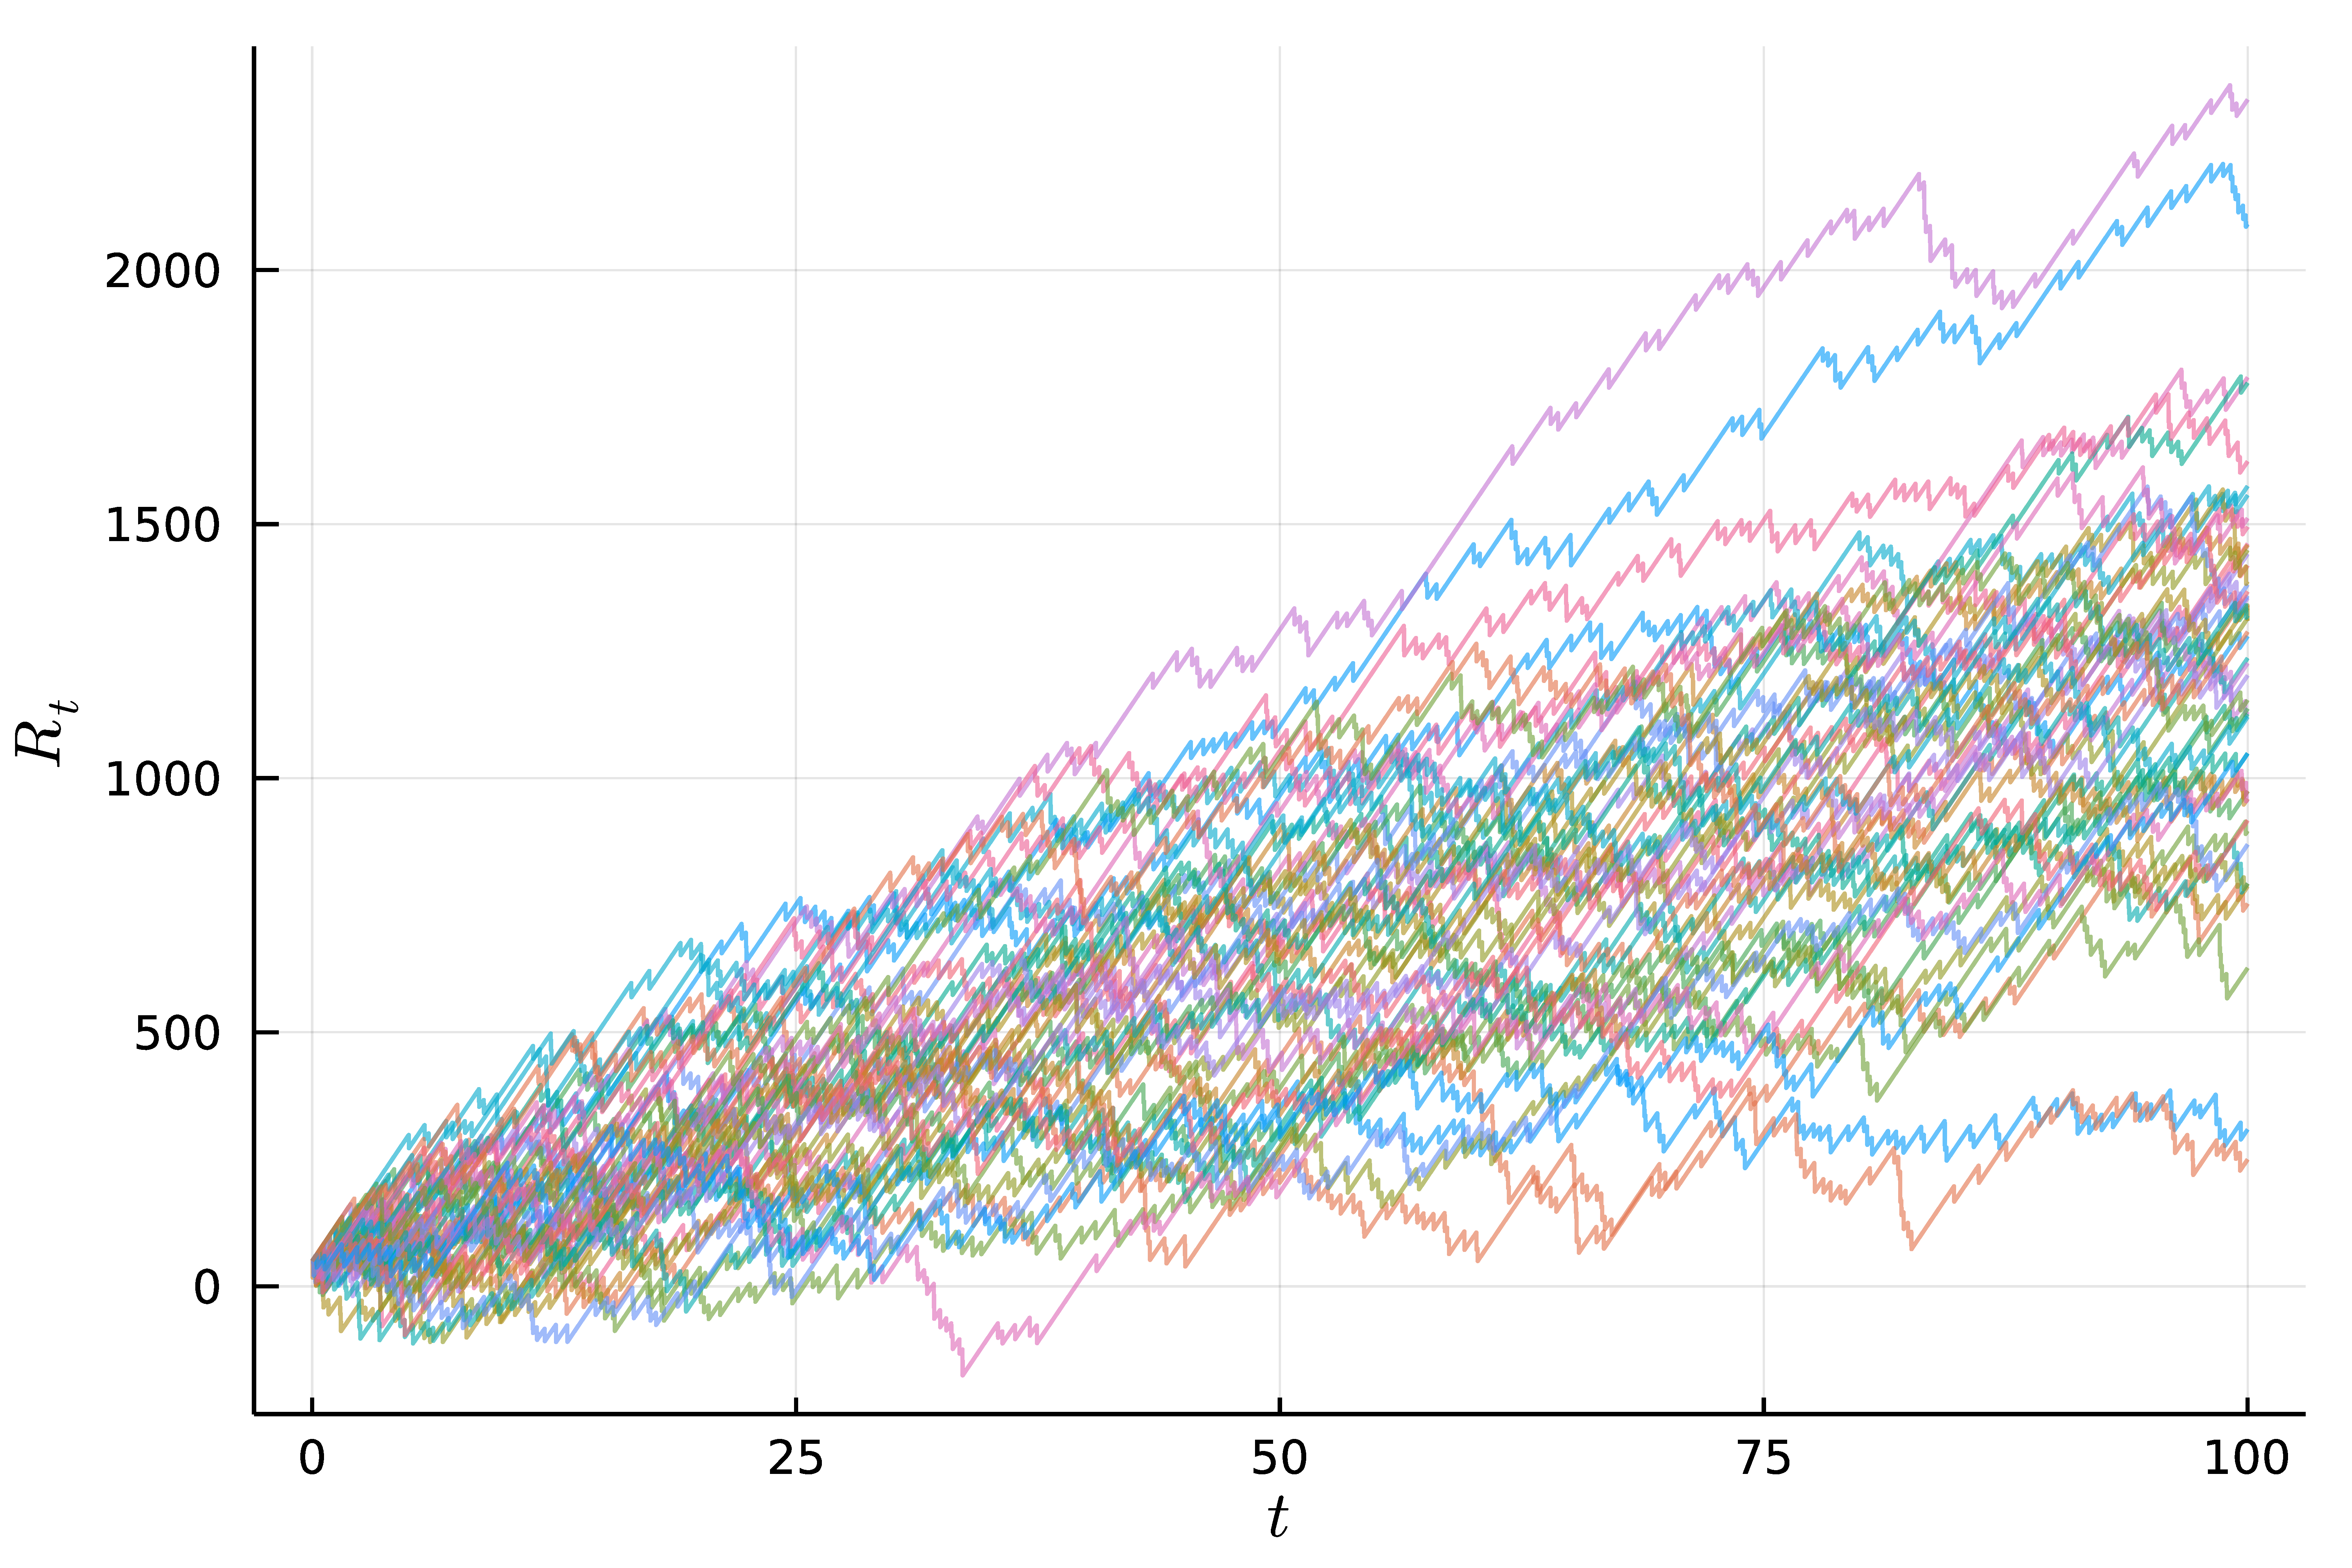
\includegraphics[width=\columnwidth]{fig/trajektorie_1.pdf}
		\caption{Trajektorie 50 realizacji klasycznego procesu Ryzyka zawartych w danych.}
	\end{figure}
	
	\subsubsection{Parametr {\boldmath $c$}}
	\noindent Możemy wyznaczyć go w bardzo prosty sposób. Wiedząc, że jest to współczynnik nachylenia funkcji liniowej $ct$, wystarczy, że policzymy o ile funkcja ta wzrasta w jednym kroku czasowym (obliczymy różnicę dwóch sąsiadujących danych) i wartość tę podzielimy przez długość kroku. Ważne, by upewnić się, czy w danym kroku nie nastąpił spadek. Dla pewności możemy policzyć $c$ dla kilku kroków i sprawdzić, czy otrzymane wartości są identyczne. Wartość, którą otrzymaliśmy z naszych danych to $c = 56,25$.
	
	\subsubsection{Parametr {\boldmath $\lambda$}}
	\noindent W przypadku tego parametru nie jesteśmy w stanie wyznaczyć jego dokładnej wartości, zatem skorzystamy z estymatora. Wykorzystamy fakt, że jeśli proces Poissona ma intensywność $\lambda$, to odstępy czasowe między kolejnymi skokami mają rozkład $\mathcal{E}xp(\lambda)$. Wydzielamy więc wszystkie czasy oczekiwania ze wszystkich trajektorii do jednego zbioru danych. Robimy to sumując wszystkie kroki czasowe następujące po każdym spadku aż do następnego spadku, przy czym dodajemy także ostatni krok spadkowy. Należy zaznaczyć w tym miejscu, że pozwalamy sobie tutaj na pewne uproszczenie, ponieważ przyjmujemy, że spadek miał miejsce dokładnie pod koniec kroku spadkowego, podczas gdy w rzeczywistości miał on miejsce w jego trakcie.\vspace{1.5mm}\\
	By wyestymować parametr $\lambda$, skorzystamy z faktu, że dla $\tau \sim \mathcal{E}xp(\lambda)$ wartość oczekiwana jest równa
	$$ \mathbb{E}\tau = \frac{1}{\lambda}. $$
	Najlepszym estymatorem wartości oczekiwanej jest średnia z próby. Oznaczmy przez $\tau_1, \dots, \tau_n$ odstępy czasowe pozyskane z naszych danych. Estymatorem $\lambda$ będzie więc
	$$ \widehat{\lambda} = \frac{1}{\frac{1}{n}\sum\limits_{i=1}^n \tau_i} = \frac{n}{\sum\limits_{i=1}^n \tau_i}. $$
	Po obliczeniu otrzymaliśmy $\widehat{\lambda} \approx 1,48$. Poniżej możemy zobaczyć, że krzywa gęstości teoretycznej rozkładu $\mathcal{E}xp\left(\widehat{\lambda}\right)$ wyraźnie pokrywa się z histogramem z naszych danych.
	
	\begin{figure}[H]
		\centering
		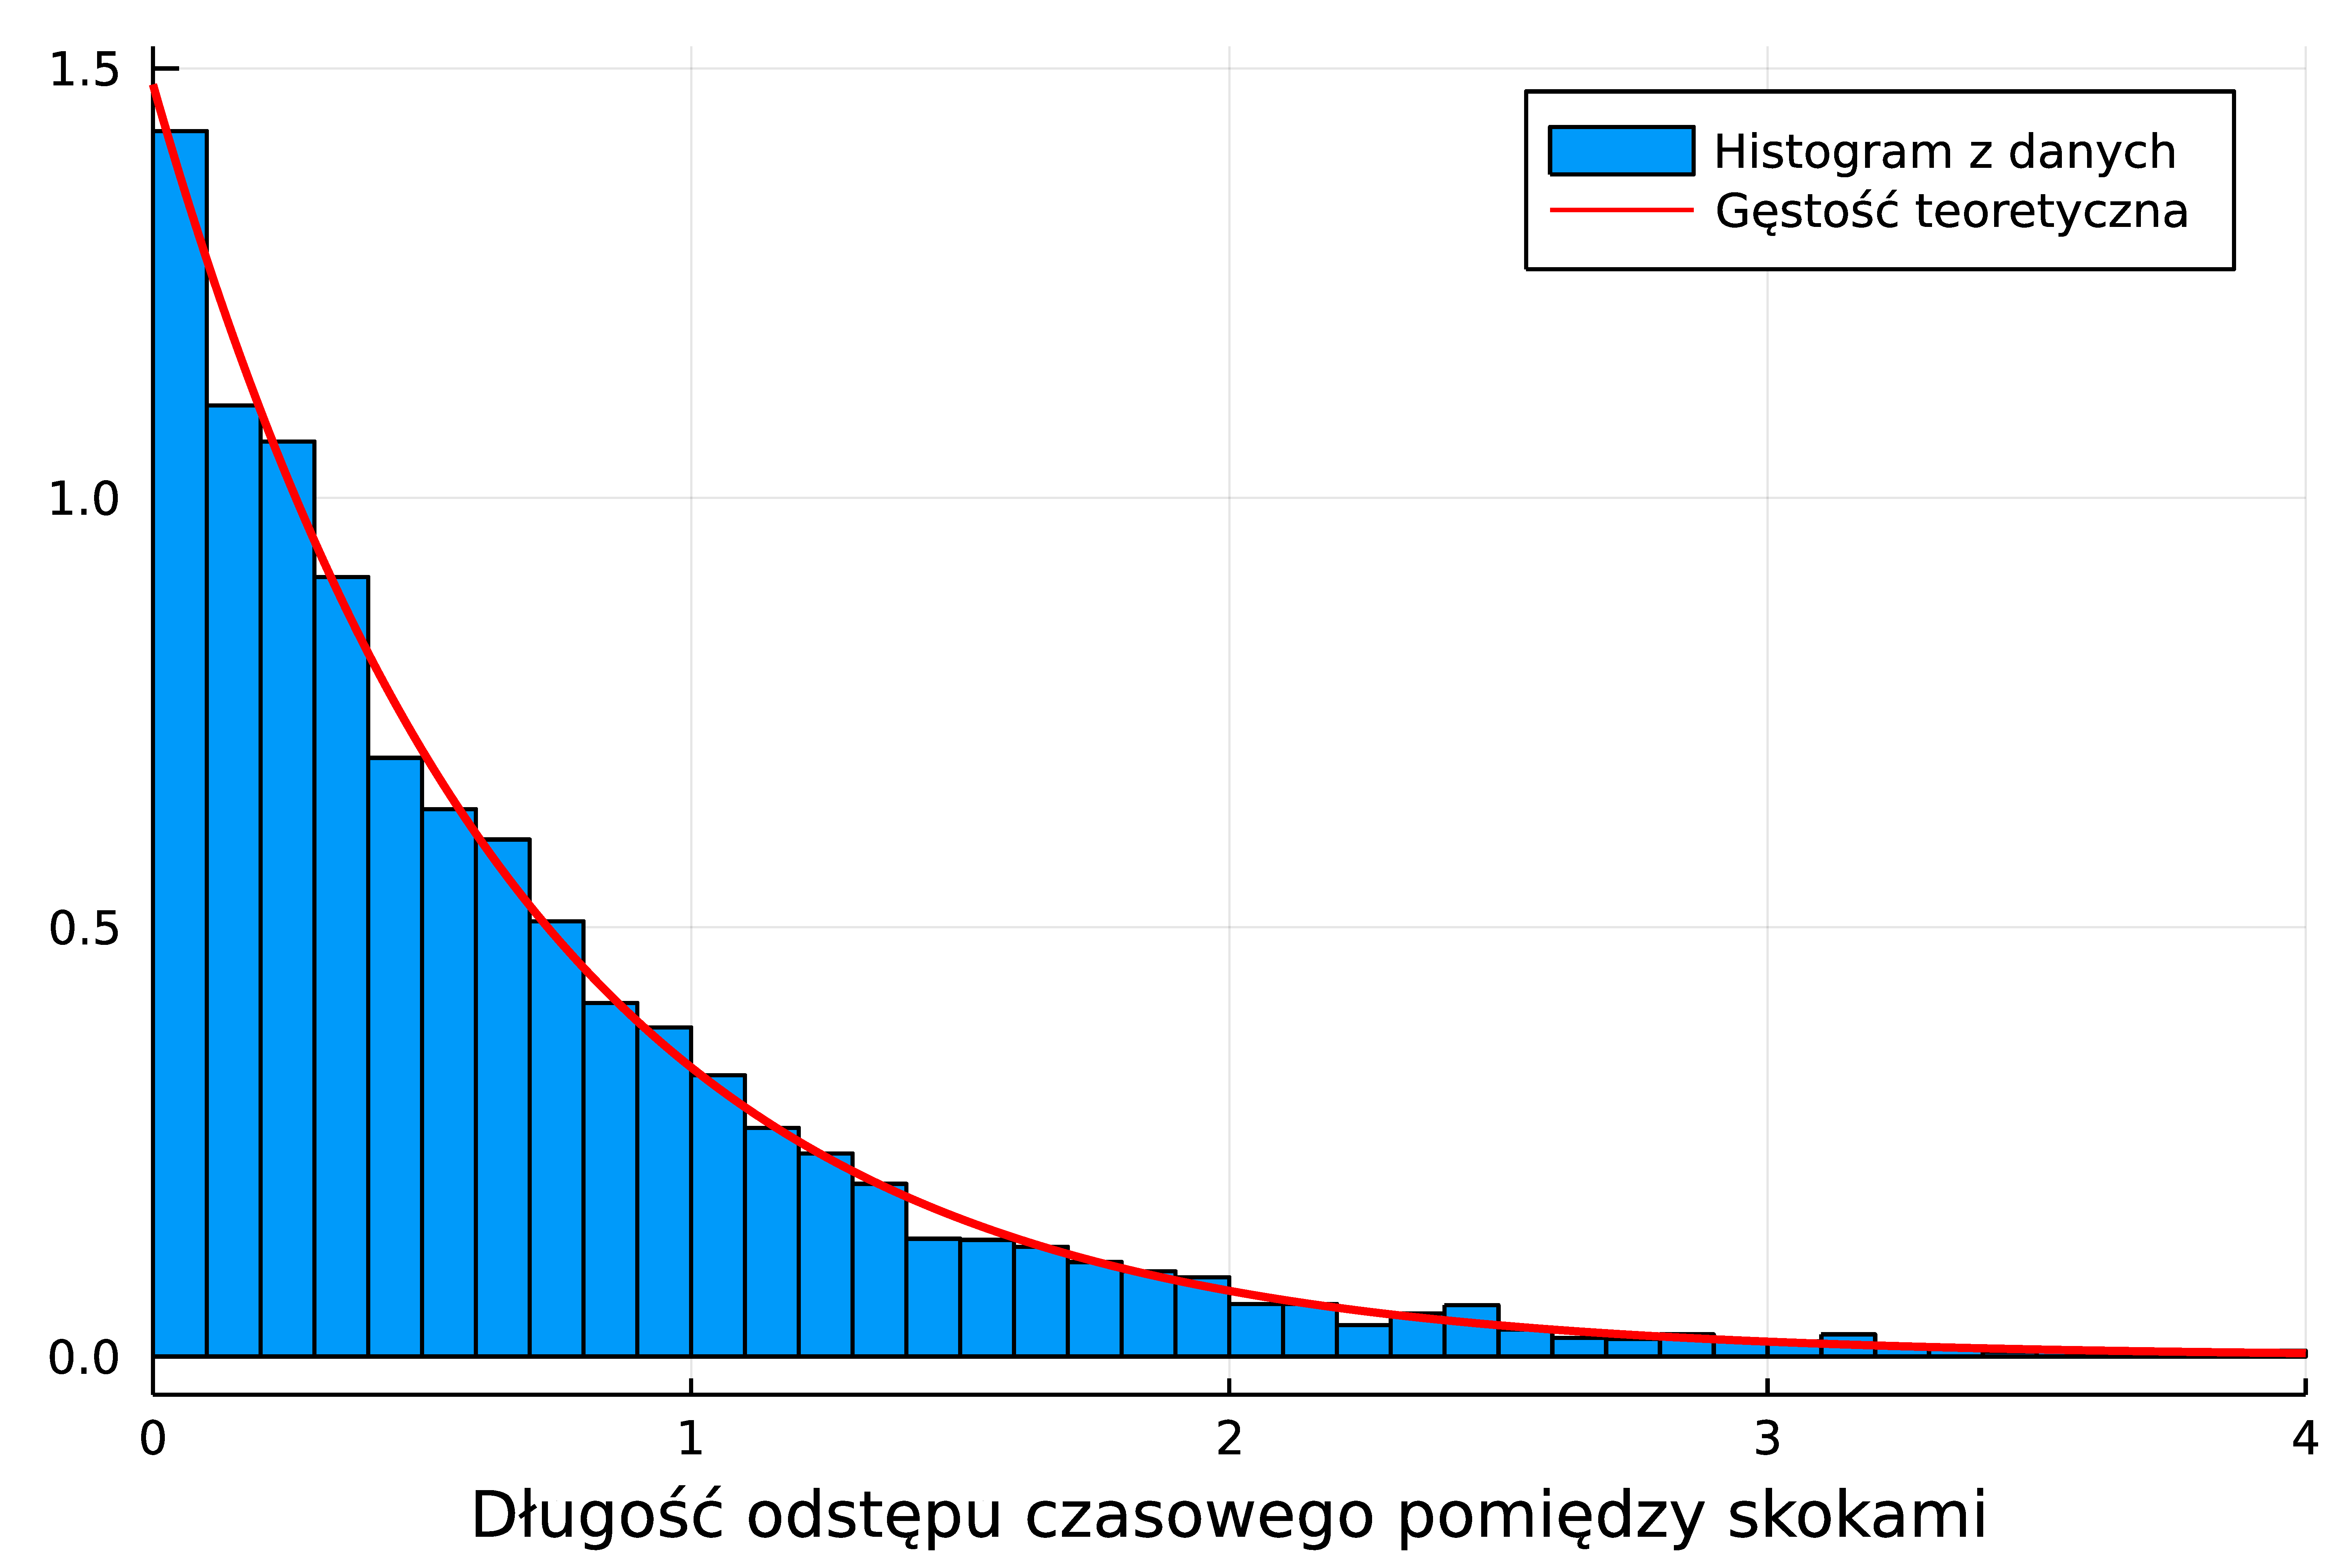
\includegraphics[width=\columnwidth]{fig/lambda.pdf}
		\caption{Porównanie unormowanego histogramu z odstępów czasowych pomiędzy skokami z gęstością teoretyczną rozkładu $\mathcal{E}xp\left(\widehat{\lambda}\right)$.}
	\end{figure}
	
	\subsubsection{Straty {\boldmath $X_i$}}
	\noindent Niezbędną informacją potrzebną do dopasowania modelu do badanego procesu Ryzyka jest rozkład strat $X_i$. Aby pozyskać dane opisujące straty, obliczamy różnicę sąsiadujących danych w każdym kroku spadkowym. Dodatkowo, ponieważ nasze dane opisują trajektorie z dokładnością do kroku czasowego, to należy do otrzymanych wartości dodać jeszcze przyrost z przychodów w tym kroku. W naszym przypadku przyrost ten będzie wynosił $c \cdot h = 0,56625$.
	
	\begin{figure}[H]
		\centering
		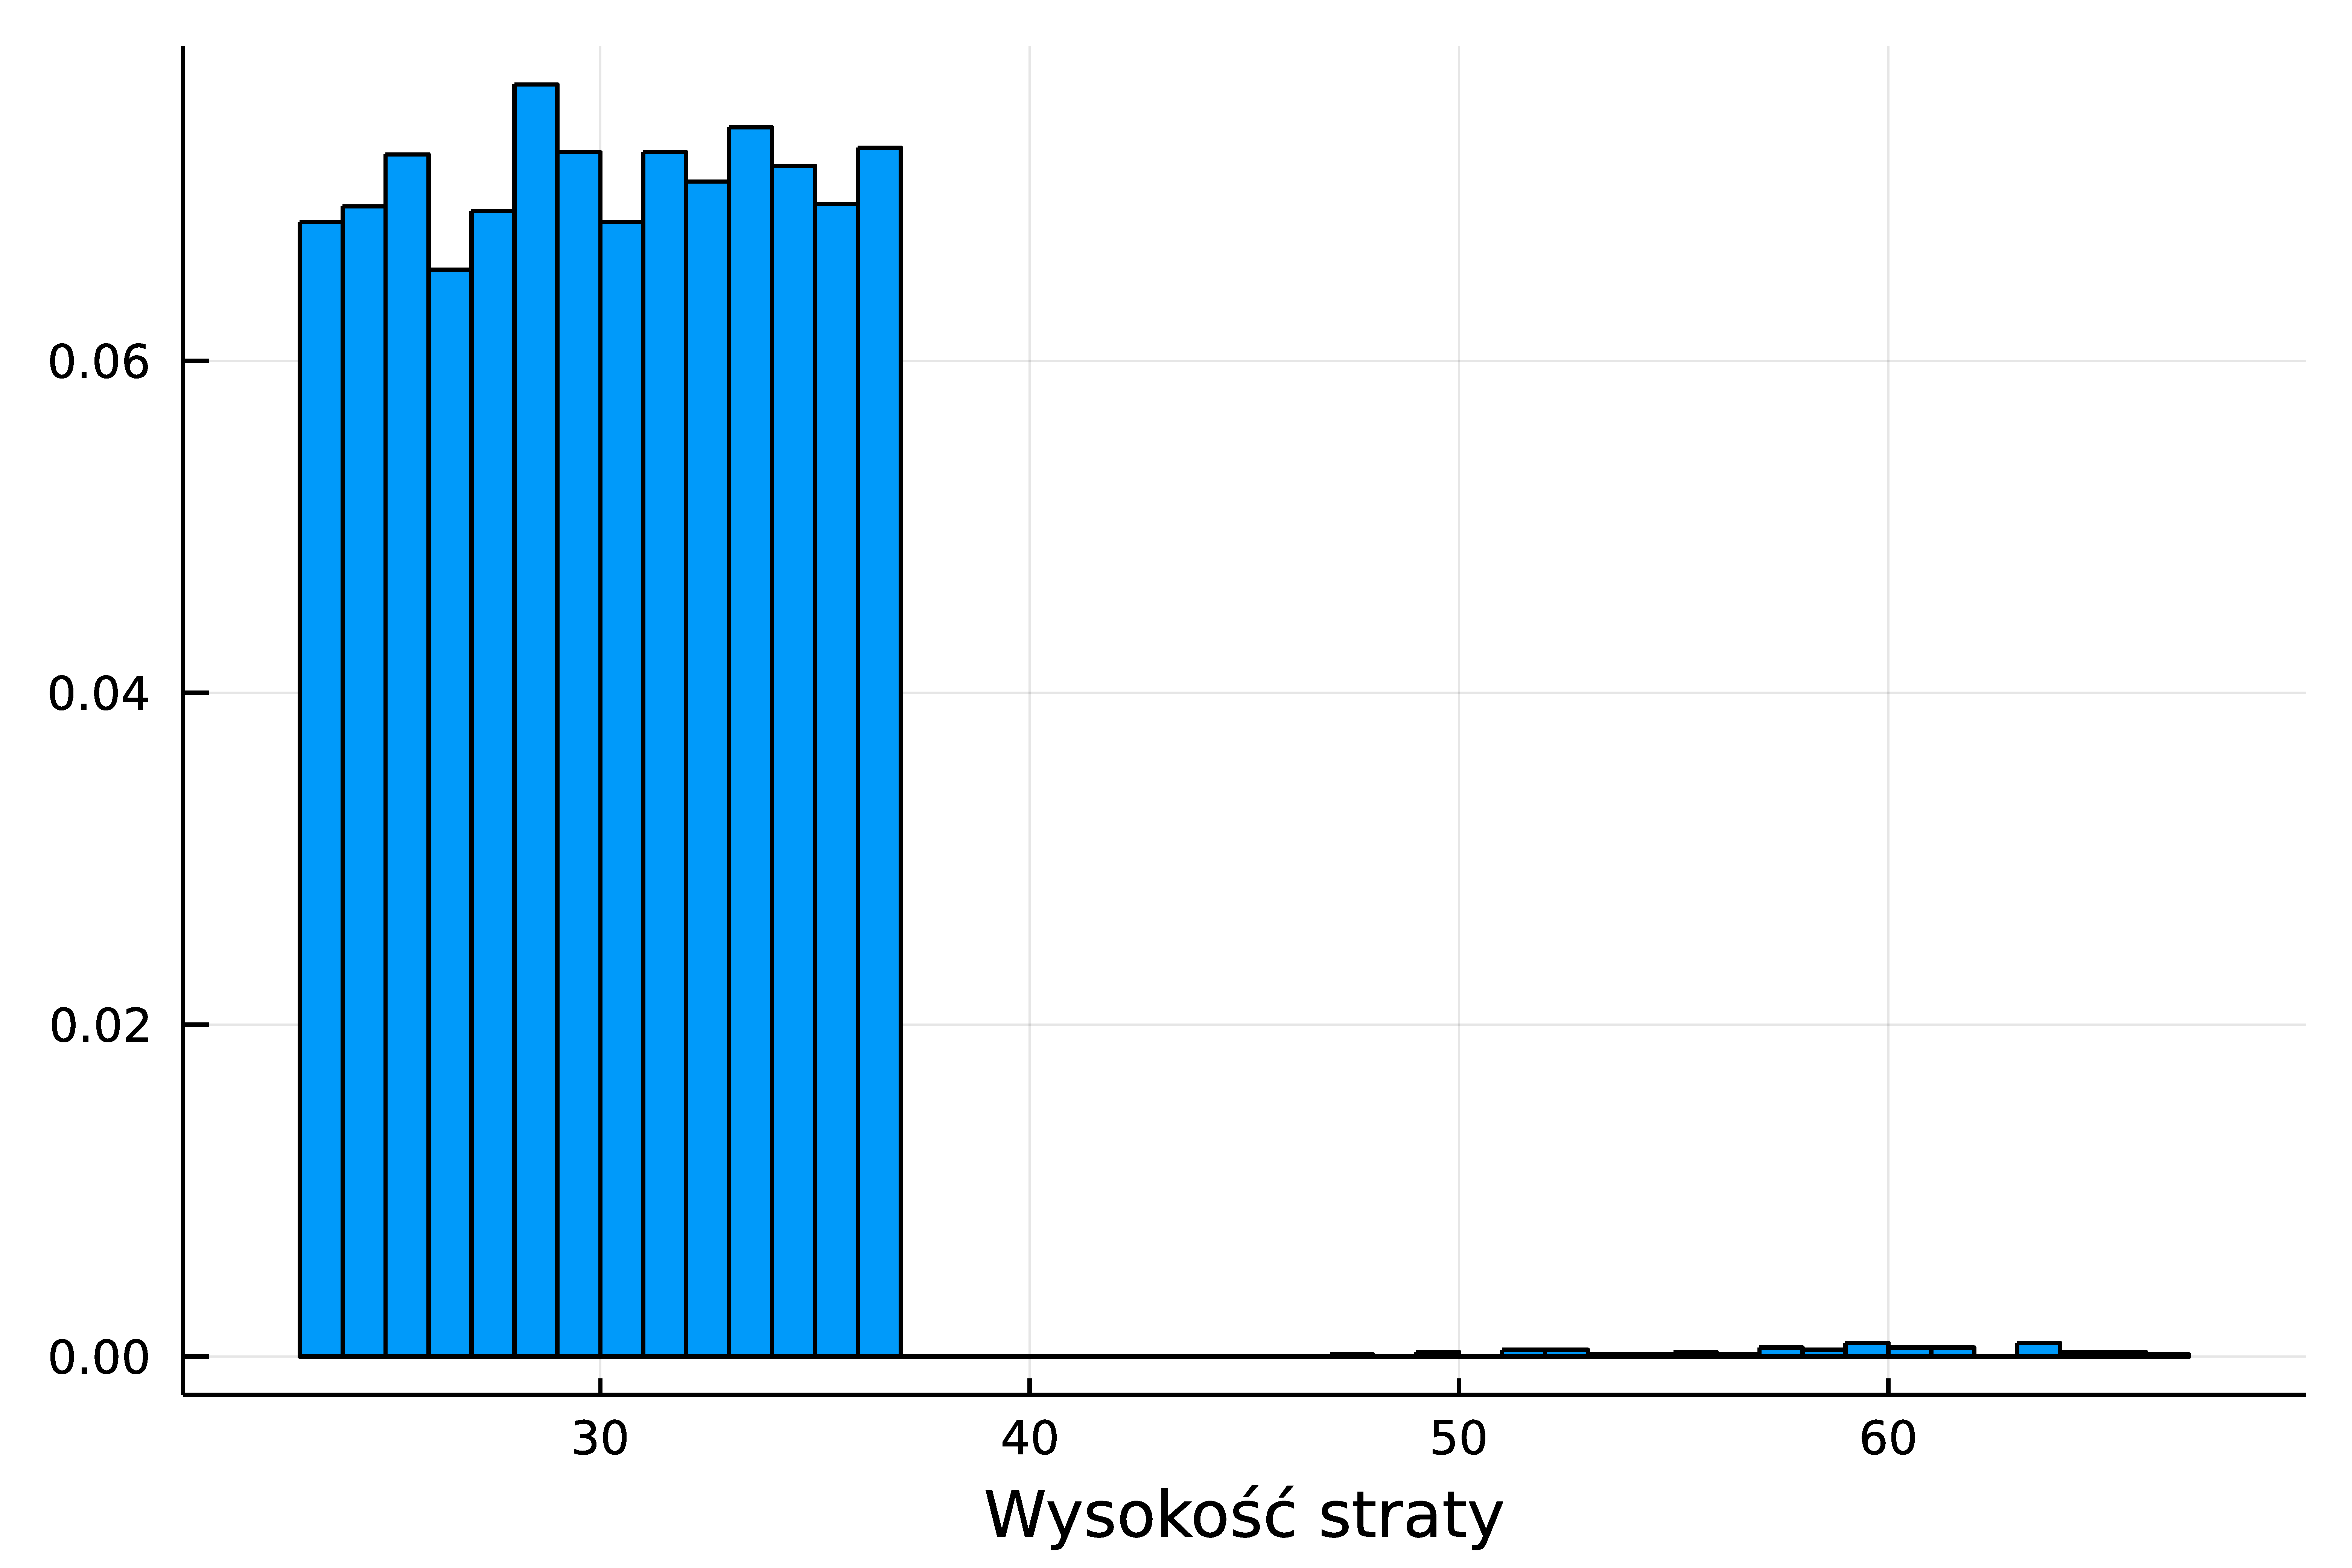
\includegraphics[width=\columnwidth]{fig/straty_1.pdf}
		\caption{Unormowany histogram ze wszystkich strat pozyskanych z 50 trajektorii.}
	\end{figure}

	\noindent Na powyższym histogramie widzimy, że zdecydowana większość danych znajduje się w okolicach 30. Kształt histogramu sugeruje, że mają one rozkład jednostajny. Możemy jednak zauważyć, że pojawia się niewielka ilość odstających większych wartości. Stąd możemy przypuszczać, że jest to kompozycja rozkładów. Zdefiniujmy zatem jej gęstość jako
	\begin{equation}\label{gęstość_strat}
		f_X(x) = p_1 f_1(x) + p_2 f_2(x),
	\end{equation}
	gdzie $p_1$ i $p_2$ są pewnymi prawdopodobieństwami ($p_1 + p_2 = 1$), a $f_1$ i $f_2$ są gęstościami skomponowanych rozkładów.
	\vspace{1.5mm}\\
	Zajmijmy się najpierw znalezieniem rozkładu dominujących danych (o gęstości $f_1$). Jak zostało wspomniane, histogram sugeruje, że mają one rozkład jednostajny. Odseparujemy te wartości definiując zbiór
	$$ K_1 = \left\{ X_i: X_i < 40 \right\}. $$
	Załóżmy, że dane te pochodzą z rozkładu $\mathcal{U}(a, b)$. Estymatorami parametrów $a$ i $b$ wyznaczonymi metodą Największej Wiarygodności są
	$$ \widehat{a} = \min(K_1) \approx 23, \ \ \widehat{b} = \max(K_1) \approx 37. $$
	Skorzystamy z testu Kołmogorowa-Smirnowa w celu weryfikacji hipotezy
	$$ H_0: X \sim \mathcal{U}(23, 37) \ \ \forall_{X \in K_1}. $$
	Otrzymaliśmy p-wartość równą $0,2449$, zatem możemy śmiało przyjąć tę hipotezę.
	\vspace{1.5mm}\\
	Pozostało nam wyznaczyć rozkład wartości odstających. Ponieważ jest ich zaledwie 46 na 7358 wszystkich danych, to nie jesteśmy w stanie jednoznacznie stwierdzić do jakiego rozkładu one należą. Jednakże, ze względu na tak niewielką ilość, nie jest to na tyle istotne, ponieważ wartości te mają marginalny wpływ na całkowity rozkład. Ważne jest, by w naszym modelu z taką samą częstością pojawiały się takie właśnie ekstremalne spadki, a ich wartość była zbliżona do tych, które zawierają dane.
	\vspace{1.5mm}\\
	Zdefiniujmy zbiór wartości odstających jako
	$$ K_2 = \left\{ X_i: X_i > 40 \right\}. $$
	
	\begin{figure}[H]\label{odstające}
		\centering
		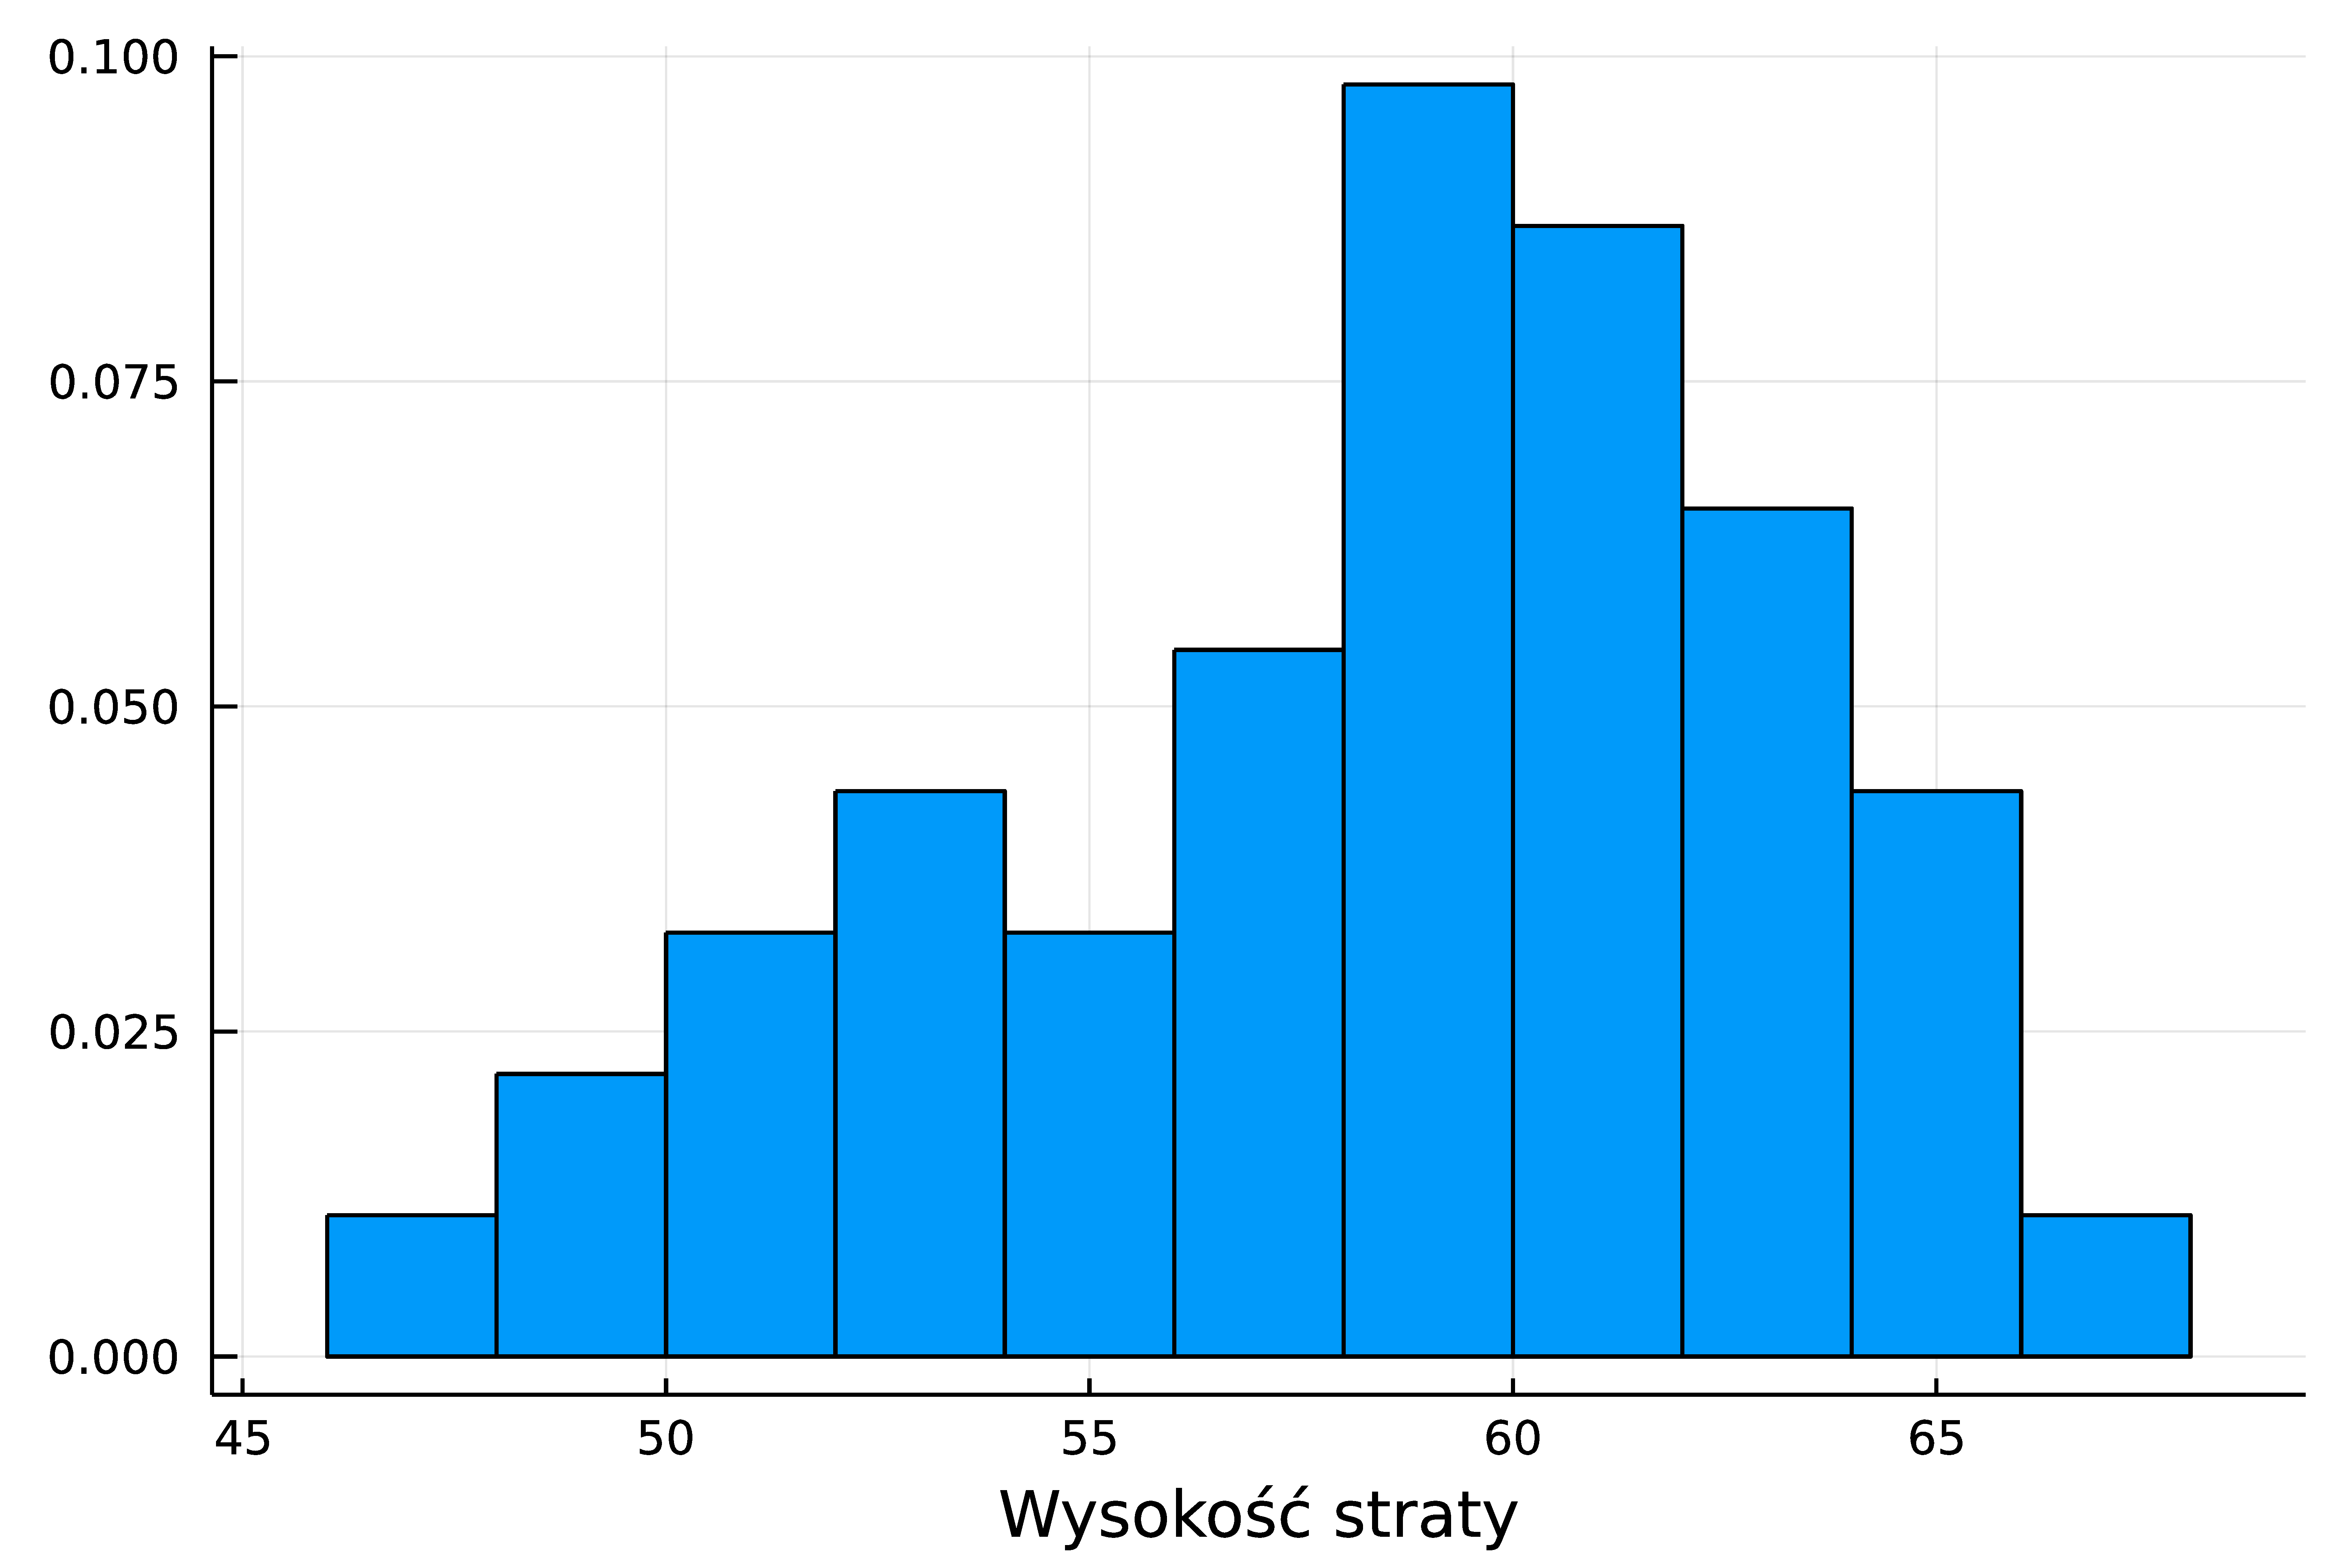
\includegraphics[width=\columnwidth]{fig/straty_2.pdf}
		\caption{Unormowany histogram ze strat większych od 40.}
	\end{figure}

	\noindent Na powyższym histogramie zauważyć możemy, że dane zachowują się w miarę podobny sposób jak rozkład normalny. Przyjmijmy więc, że
	$$ X \sim \mathcal{N}(m, \sigma^2) \ \ \forall_{X \in K_2}. $$
	Estymatorami parametrów $m$ i $\sigma^2$ są oczywiście
	$$ \widehat{m} = \frac{1}{\mathrm{\#}K_2}\sum_{X \in K_2} X \approx 58,5\ , \ \ \ \widehat{\sigma}^2 = \frac{1}{\#K_2 - 1}\sum_{X \in K_2} (X - \widehat{m})^2 \approx 4,88. $$
	Dla tego rozkładu również przeprowadziliśmy test Kołmogorowa-Smirnowa i otrzymaliśmy p-wartość równą $0,7586$, więc możemy zaakceptować nasze założenie.
	\vspace{1.5mm}\\
	Policzmy jeszcze współczynniki $p_1$ i $p_2$ we wzorze \eqref{gęstość_strat}.
	Możemy je wyestymować w prosty sposób:
	$$ \widehat{p}_1 = \frac{\#K_1}{\#K_1 + \#K_2} \approx 0,9937\ , \ \ \ \widehat{p}_2 = \frac{\#K_2}{\#K_1 + \#K_2} \approx 0,0063. $$
	Na koniec znajdźmy wartość parametru $\mu$. Wystarczy, że obliczymy średnią ze wszystkich strat, czyli
	$$ \widehat{\mu} = \frac{1}{n} \sum_{i=1}^n X_i \approx 30,23. $$

	
	\subsubsection{Parametr {\boldmath $\theta$}}
	\noindent Znając już wszystkie parametry z prosty sposób możemy wyliczyć wartość parametru $\theta$ odpowiadającego za wysokość premii. Przekształcając wzór \eqref{c} dostaniemy
	$$ \theta = \frac{c}{\mu\lambda} - 1. $$
	Po podstawieniu wartości otrzymujemy $\theta \approx 0,256$.
	
	
	
	\subsubsection{Gotowy model}
	\noindent Po wyznaczeniu wszystkich potrzebnych parametrów i znalezieniu rozkładu strat możemy sprawdzić działanie modelu. Zanim to zrobimy, wyznaczmy średnią procesu. Jest funkcja liniowa postaci
	\begin{multline*}
		m(t) = \mathbb{E}R_t = \mathbb{E}\left[u + ct - \sum_{i=1}^{N_t} X_i \right] = u + ct + \mathbb{E}\left[ \mathbb{E}\left[ \sum_{i=1}^{N_t} X_i | N_t \right] \right]\\ = u + ct - \mu\lambda t = u + (1 + \theta)\mu\lambda t - \mu\lambda t = u + \mu\lambda\theta t.
	\end{multline*}
	
	\begin{figure}[H]
		\centering
		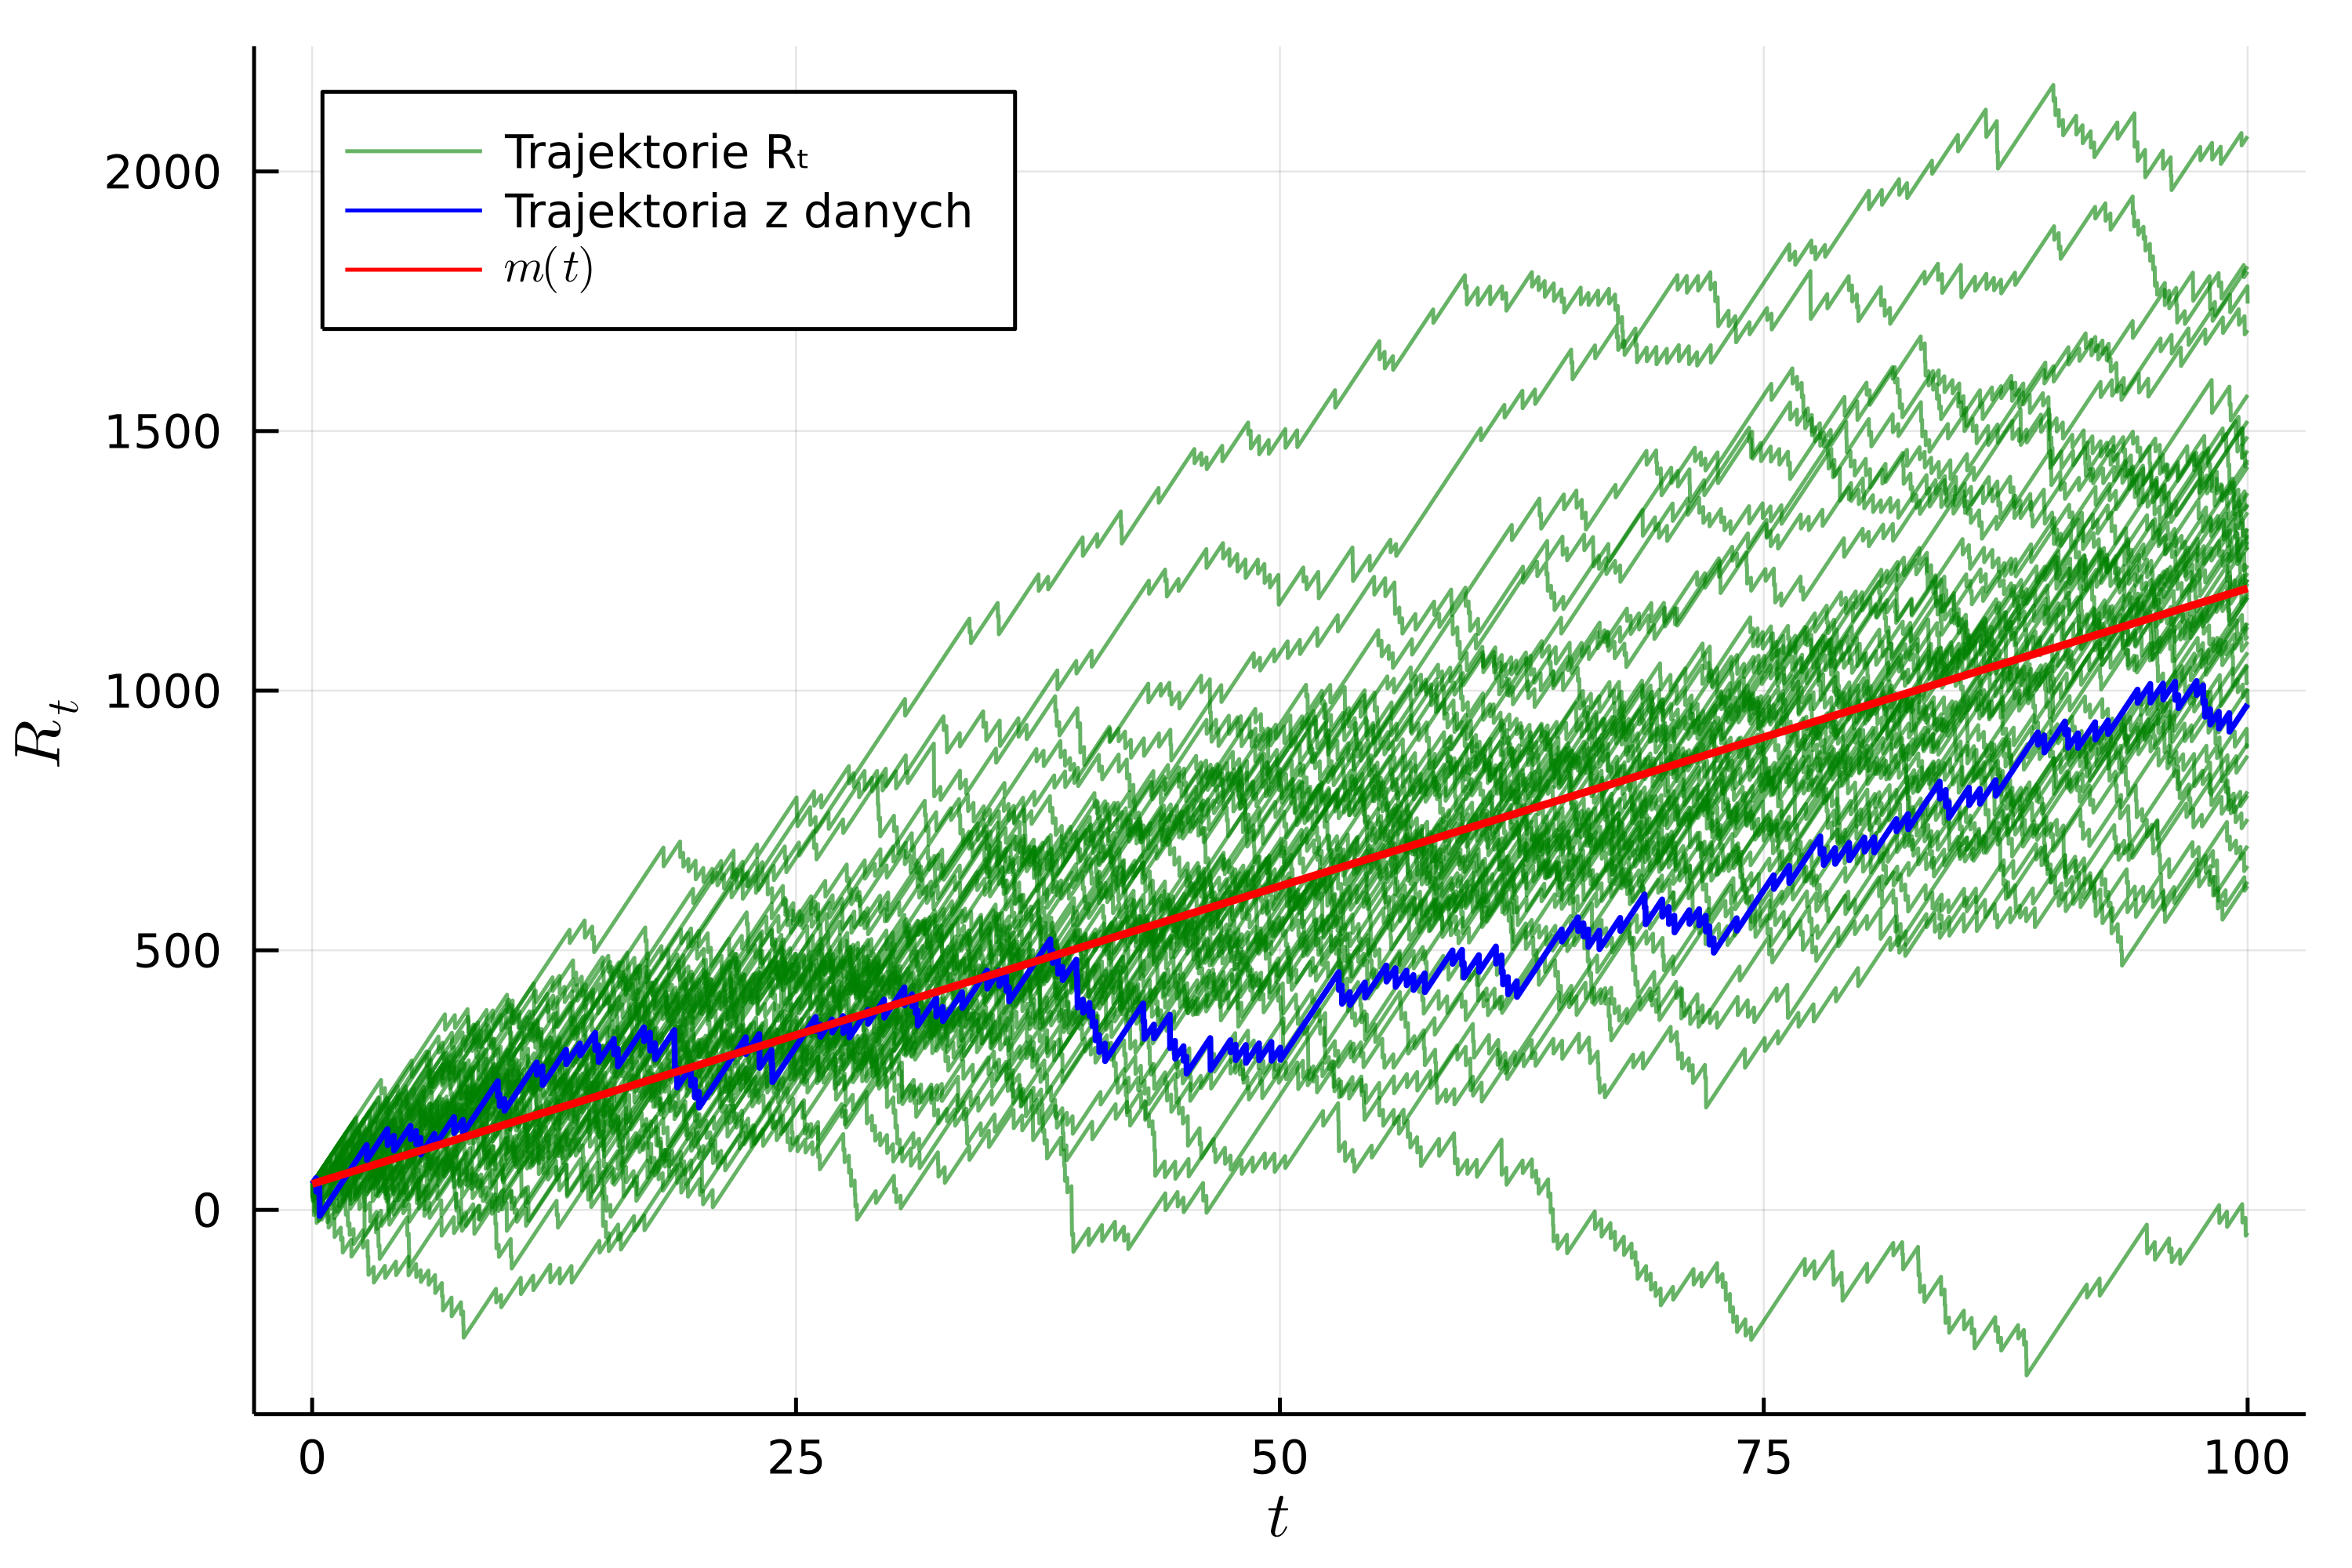
\includegraphics[width=\columnwidth]{fig/trajektorie_2.png}
		\caption{Wykres 100 trajektorii klasycznego modelu Ryzyka z wyznaczonymi parametrami wraz z jedną trajektorią z danych oraz średnią procesu wyznaczoną analitycznie.}
		\label{fig:trajektorie2}
	\end{figure}

	\begin{figure}[H]
		\centering
		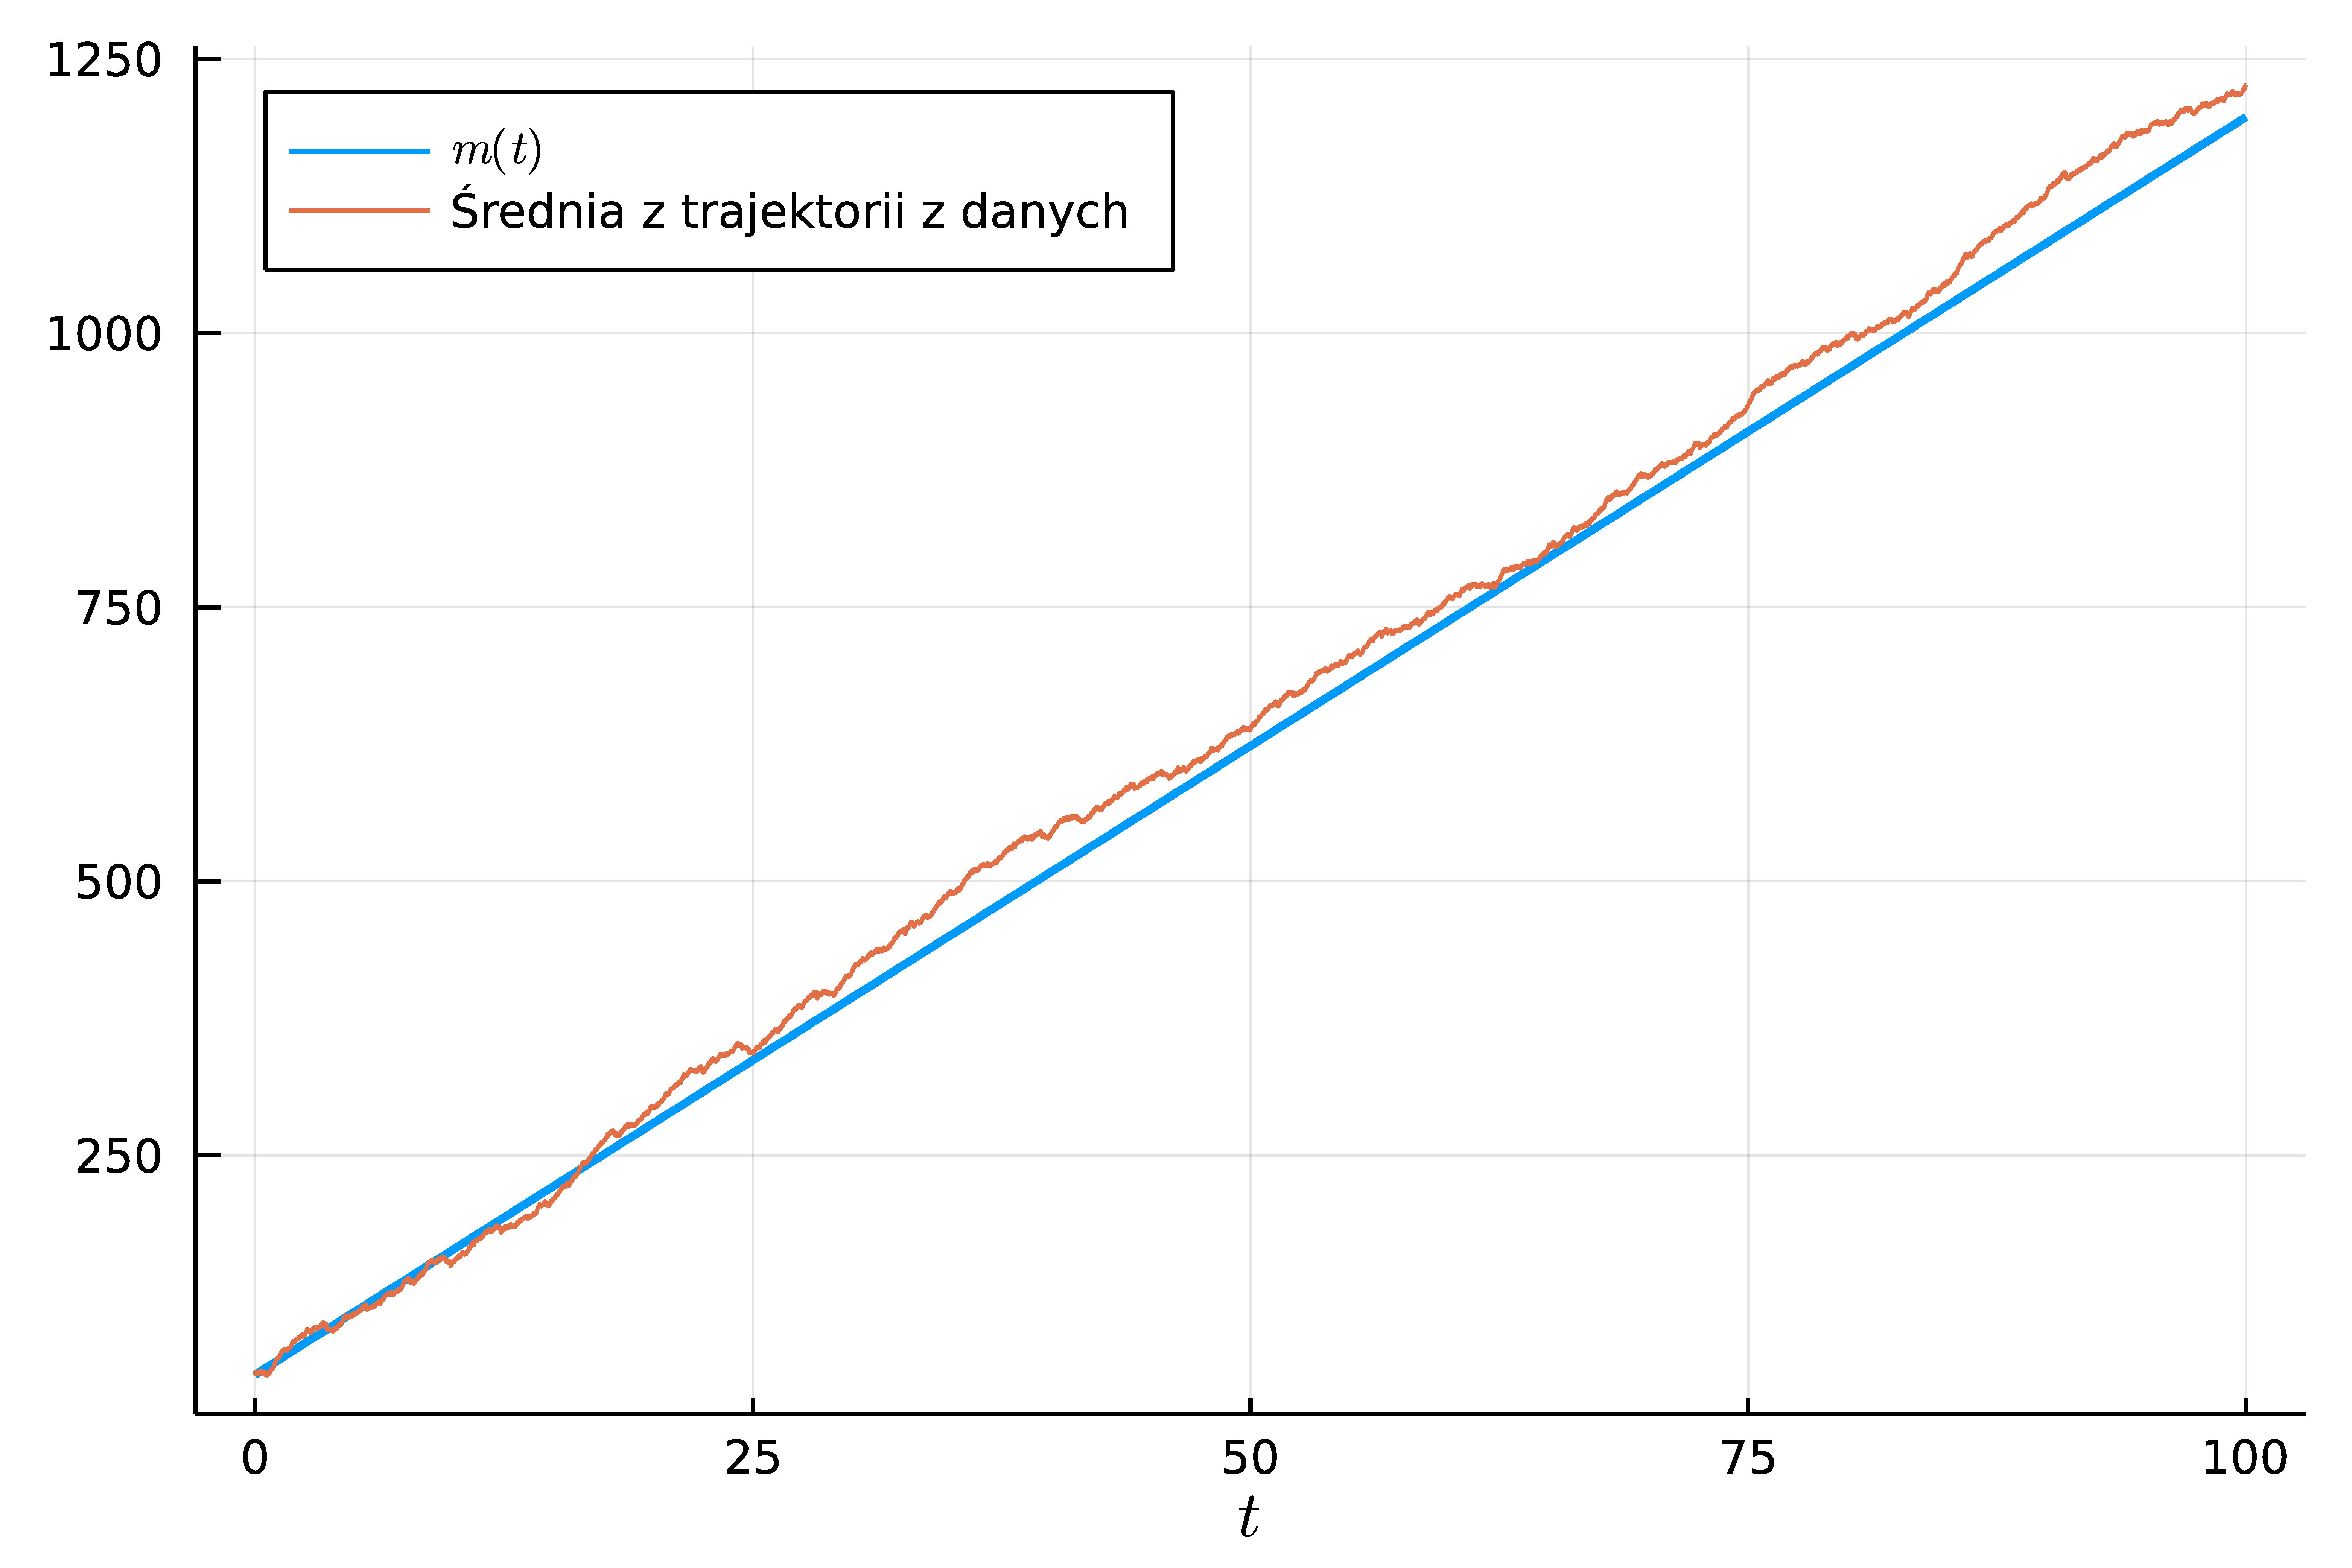
\includegraphics[width=\columnwidth]{fig/srednia_porownanie.pdf}
		\caption{Porównanie funkcji średniej $m(t)$ wyznaczonego procesu oraz średniej z trajektorii z danych.}
		\label{fig:średnia}
	\end{figure}

	\noindent Jak widzimy na Rys. \ref{fig:trajektorie2}, wysymulowane trajektorie oscylują wokół średniej procesu. Pojedyncza trajektoria pochodząca z danych wydaje się zachowywać podobnie do tych wysymulowanych. Z kolei na Rys. \ref{fig:średnia} można zobaczyć, że funkcja średniej $m(t)$ dla naszego procesu pokrywa się ze średnią z trajektorii, które zawierają dane.
	
	
	
	\subsection{Prawdopodobieństwo ruiny}
	\noindent Gdy już udało nam się wydobyć z danych wszystkie potrzebne informacje aby dopasować do nich nasz model, możemy rozpocząć analizę wyznaczonego procesu. Naszym celem jest obliczenie prawdopodobieństwa ruiny (bankructwa) firmy, dla której może być to najcenniejsza informacja, ponieważ pokazuje jakie są szanse, że firma odniesie sukces.
	
	\subsubsection{Prawdopodobieństwo ruiny w skończonym czasie}
	\noindent Definiujemy moment ruiny jako
	$$ \tau(u) = \inf\{t \geq 0: \ R_t < 0\}, $$
	gdzie $u$ oznacza kapitał początkowy. Prawdopodobieństwo ruiny w skończonym czasie $T$ definiujemy poprzez
	$$ \Psi(u, T) = \mathbb{P}(\tau(u) < T). $$
	Prawdopodobieństwo to da się wyznaczyć tylko w przypadku, gdy $X_i$ mają rozkład wykładniczy, co nas nie dotyczy. Skorzystamy więc z symulacji Monte Carlo.\\
	
	\noindent \textbf{Algorytm}
	\begin{enumerate}[leftmargin=10mm]
		\item Generuj $N$ trajektorii $R_t^{(1)}, \dots, R_t^{(N)}$ procesu ryzyka na $[0, T]$.
		\item Wyznacz $ n = \#\left\{ i = 1,\dots,N: \min\limits_{t \in [0, T]} R_t^{(i)} < 0 \right\} $.
		\item Zwróć $\Psi(u, T) = \frac{n}{N}$.
	\end{enumerate}
	Wygenerowaliśmy więc $N = 10\ 000$ trajektorii na przedziałach $[0, 100]$ i $[0, 200]$, po czym sprawdziliśmy ile z nich spadło w dowolnym momencie poniżej zera. Otrzymaliśmy
	$$ \Psi(50, 100) = 0,409 \ , \ \ \ \Psi(50, 200) = 0,4194 .$$
	
	\subsubsection{Prawdopodobieństwo ruiny w nieskończonym czasie}
	\noindent Definiujemy prawdopodobieństwo ruiny w nieskończonym czasie jako
	$$ \Psi(u) = \mathbb{P}(\tau(u) < \infty). $$
	Analityczne wyznaczenie $\Psi(u)$ także nie jest możliwe w naszym przypadku. Nie możemy również skorzystać z metody Monte Carlo, ponieważ czas jest tym razem nieskończony. Posłużymy się więc wzorem Pollaczka-Chinczyna, który wygląda następująco:
	$$ \Psi(u) = \frac{\theta}{1 + \theta} \sum_{n=0}^{\infty} \left( \frac{1}{1 + \theta} \right)^n B_n(u), $$
	gdzie $B_n(u) = \mathbb{P}(Y_1 + \dots + Y_n > u)$ i $Y_i$ to zmienne losowe iid o gęstości \mbox{$f(x) = \frac{1 - F_X(x)}{\mu}$}, $x > 0$, a $F_X(x)$ jest dystrybuantą rozkładu strat $X_i$. Wykorzystamy pewien fakt wynikający z tego wzoru, a konkretnie to, że
	$$ \Psi(u) = \mathbb{P}(Y_1 + \dots + Y_K > u), $$
	gdzie $K \sim \mathcal{G}eom \left( \frac{\theta}{1+\theta} \right)$.\\
	
	\noindent \textbf{Algorytm}
	\begin{enumerate}[leftmargin=10mm]
		\item Definiuj $Z = 0$.
		\item Generuj $K \sim \mathcal{G}eom \left( \frac{\theta}{1+\theta} \right)$.
		\item Generuj $Y_1, \dots, Y_K$ z rozkładu o gęstości $f(x) = \frac{1 - F_X(x)}{\mu}, \ x > 0$.
		\item Jeśli $Y_1 + \dots + Y_K > u$, to $Z = Z + 1$.
		\item Kroki 2, 3, 4 powtórz $N$ razy.
		\item Zwróć $\Psi(u) = \frac{Z}{N}$.
	\end{enumerate}
	Zauważmy, że do tej symulacji potrzebna jest nam gęstość $f(x) = \frac{1 - F_X(x)}{\mu}$. Ponieważ $F_X$, czyli dystrybuanta rozkładu zmiennych $X_i$ jest kompozycją dwóch innych dystrybuant (podobnie jak dla gęstości we wzorze \eqref{gęstość_strat}), w tym dystrybuanty rozkładu normalnego, wyznaczenie gęstości $f$ będzie problematyczne. Wiemy jednak, że współczynnik $p_2$ jest bardzo mały, a więc możemy pozwolić sobie na małe uproszczenie i w symulacji uwzględnić tylko dystrybuantę rozkładu jednostajnego, czyli
	$$ F_1(x) = \begin{cases}
		0, & x < 23 \\
		\frac{x - 23}{14}, & 23 \leq x < 37 \\
		1, & 37 \leq x
	\end{cases}. $$
	Wtedy musimy także przyjąć wartość teoretyczną $\mu$ dla tego rozkładu tzn. $\mu = 30$. Po takim uproszczeniu otrzymamy 
	$$ f(x) = \begin{cases}
		0, & x < 0 \\
		\frac{1}{30}, & 0 \leq x < 23 \\
		\frac{37 - x}{420}, & 23 \leq x < 37\\
		0, & 37 \leq x
		\end{cases}. $$
	Zmienne o takiej gęstości już o wiele łatwiej wygenerować (np. metodą akceptacji i odrzucenia). Ostatecznie po wykonaniu algorytmu dla $N = 1\ 000\ 000$ powtórzeń, otrzymaliśmy
	$$ \Psi(50) \approx 0,4206.$$
	Wynik ten może być odrobinę zaniżony przez to, że nie uwzględniliśmy odstających wartości. Mimo to jest on większy od poprzednich prawdopodobieństw dla skończonego czasu, co jest naturalne, ponieważ im więcej czasu minie, tym więcej trajektorii może jeszcze spaść do zera.
	
	
	\section{Zadanie 2}
	\subsection{Proces Wienera}
	\noindent Procesem Wienera (Ruchem Browna) nazywamy proces $\{W_t\}_{t\geqslant0}$, który spełnia następujące własności:
	\begin{itemize}[leftmargin=10mm, label=\small$\bullet$]%label=$\boldsymbol{\cdot}$]
		\item $W_0=0$,
		\item $W_t$ ma niezależne przyrosty,
		\item $W_t$ ma stacjonarne przyrosty,
		\item $W_t \sim \mathcal{N}(0, t)$,
		\item $W_t$ ma ciągłe trajektorie.
	\end{itemize}	
	\noindent \textbf{Algorytm}\\
	\noindent Naszym celem jest wygenerowanie wektora $\left[W_{t_0}, W_{t_1}, \dots, W_{t_n}\right]$, gdzie
%	\begin{equation*}
%		t_i=ih, \quad i=0,1,\dots,n, \quad h=T/n
%	\end{equation*}
	\begin{equation*}
		t_i=ih, \quad i\in\left[n\right]=\left\{0, 1, \dots, n\right\}, \quad h=T/n
	\end{equation*}
%	\begin{equation*}
%		t_i=ih, \quad i\in\mathbb{N}_0^{\leqslant n}, \quad h=T/n.
%	\end{equation*}
	W tym celu stosujemy poniższy algorytm
	\begin{enumerate}[leftmargin=10mm]
		\item Generuj realizację zmiennych $\xi_i\text{ iid. }\mathcal{N}(0,1), \,i\in\left[n-1\right]$,
		\item $W_{t_0}=W\left(0\right)=0$,
		\item $W_{t_{i+1}} = W_{t_{i}}+\sqrt{h}\xi_i,\quad i\in\left[n-1\right]$%\in\mathbb{N}^{n}$.
	\end{enumerate}

	\subsection{Czas wyjścia}
	\noindent Czasem wyjścia tego procesu z ustalonego przedziału $[a, b]$ nazywamy zmienną
	\begin{equation*}
		\tau=\inf\left\{t\geqslant0:W_t\notin[a, b]\right\}.
	\end{equation*}
	Niech $\left\{B^x_t\right\}_{t\geqslant0}$ będzie ruchem Browna startującym z $x\in\mathbb{R}$. Zdefiniujmy teraz zmienną 
	\begin{equation*}
		\tau^x=\inf\left\{t\geqslant0:B^x_t\notin[a, b]\right\}.
	\end{equation*}
%	dla $x$ z przedziału $[a,b]$.
	 Łatwo można pokazać, że $B^{x+y}_t\in[a ,b] \iff B^x_t\in[a-y, b-y]$.
%	\\Ponieważ $W_t+x\in[a, b] \iff W_t\in[a-x, b-x]$ \\
%	$B^x_t\in[a,b]\iff B^y_t\in[a-x+y, b-x+y]$\\widzimy, że czas wyjścia nie zależy bezpośrednio od wyboru punktów $a$ oraz $b$, a od punktu początkowego oraz długości przedziału.
	Dodatkowo, ponieważ ruch Browna jest $\frac{1}{2}$-samopodobny ($W_t\overset{d}{=}\sqrt{\Delta}W_{t/\Delta}$), zachodzi równość
	\begin{equation*}
		B^x_t=W_t+x\overset{d}{=}\Delta W_{t/\Delta^2}+x = \Delta\left(W_{t/\Delta}-\frac{x}{\Delta}\right)=\Delta B^{x/\Delta}_{t/\Delta^2}.
	\end{equation*}
	Korzystając z tych dwóch własności można udowodnić, że
	\begin{equation*}
		\begin{split}
			\tau^x&\overset{d}{=}\inf\left\{\Delta^2\frac{t}{\Delta^2}\geqslant0:\Delta B^{x/\Delta}_{t/\Delta^2}\notin[a, b]\right\} =\Delta^2\inf\left\{t^*\geqslant0:B^{x/\Delta}_{t^*}\notin\left[\frac{a}{\Delta},\frac{b}{\Delta}\right]\right\}\\
			&=\Delta^2\inf\left\{t^*\geqslant0:B^{(x-s)/\Delta}_{t^*}\notin\left[\frac{a-s}{\Delta},\frac{b-s}{\Delta}\right]\right\}.
		\end{split}
	\end{equation*}
	Wybierając teraz $\Delta=(b-a)$ oraz $s=a$ otrzymujemy
	\begin{equation}\label{eq:tau_przeskalowane}
		\tau^x\overset{d}{=}(b-a)^2\inf\left\{t\geqslant0:B^y_t\in[0,1]\right\}=(b-a)^2\widetilde\tau^y,
	\end{equation}
	gdzie $\widetilde\tau^y$ jest czasem wyjścia z przedziału $[0, 1]$ jeśli zaczniemy z punktu $y=\frac{x-a}{b-a}$, czyli z punktu dzielącego ten odcinek w stosunku takim samym jak $x$ dzieli odcinek $[a, b]$.\vspace{1.5mm}\\
	\noindent Dzięki tym przekształceniom widzimy, że $\mathbb{E}\tau^x$ zwiększa się z kwadratem długości przedziału jaki rozważamy oraz zależy ona od odległości $x$ od jednego końca przedziału względem drugiego. Z tego powodu później będziemy rozważać jedynie czas wyjścia z przedziału $[0, 1]$.
	
	
	\subsection{Średni czas wyjścia procesu Wienera}
%	\noindent Interesuje nasz średni czas wyjścia procesu w zależności od wybranego $x$. Można pokazać, że $\mathbb{E}\tau^x<\infty$\textsuperscript{\cite{art}}. Wiemy dodatkowo, że średnia w próbie jest dobrym estymatorem wartości oczekiwanej. Dlatego posłużyliśmy się tą metodą do oszacowania szukanej wartości. W wyniku otrzymaliśmy poniższy wykres
	\noindent Interesuje nasz średni czas wyjścia procesu Weinera w zależności od wybranego punktu startowego $x$. Tą wielkość oszacowaliśmy poprzez obliczenie średniej w wygenerowanej przez nas próbie. Metoda jest poprawna, ponieważ średnia w próbie jest dobrym estymatorem wartości oczekiwanej oraz można udowodnić, że $\mathbb{E}\tau^x<\infty$\textsuperscript{\cite{art}}. W wyniku symulacji otrzymaliśmy poniższy wykres
%	 W wyniku otrzymaliśmy poniższy wykres
	\begin{figure}[H]
		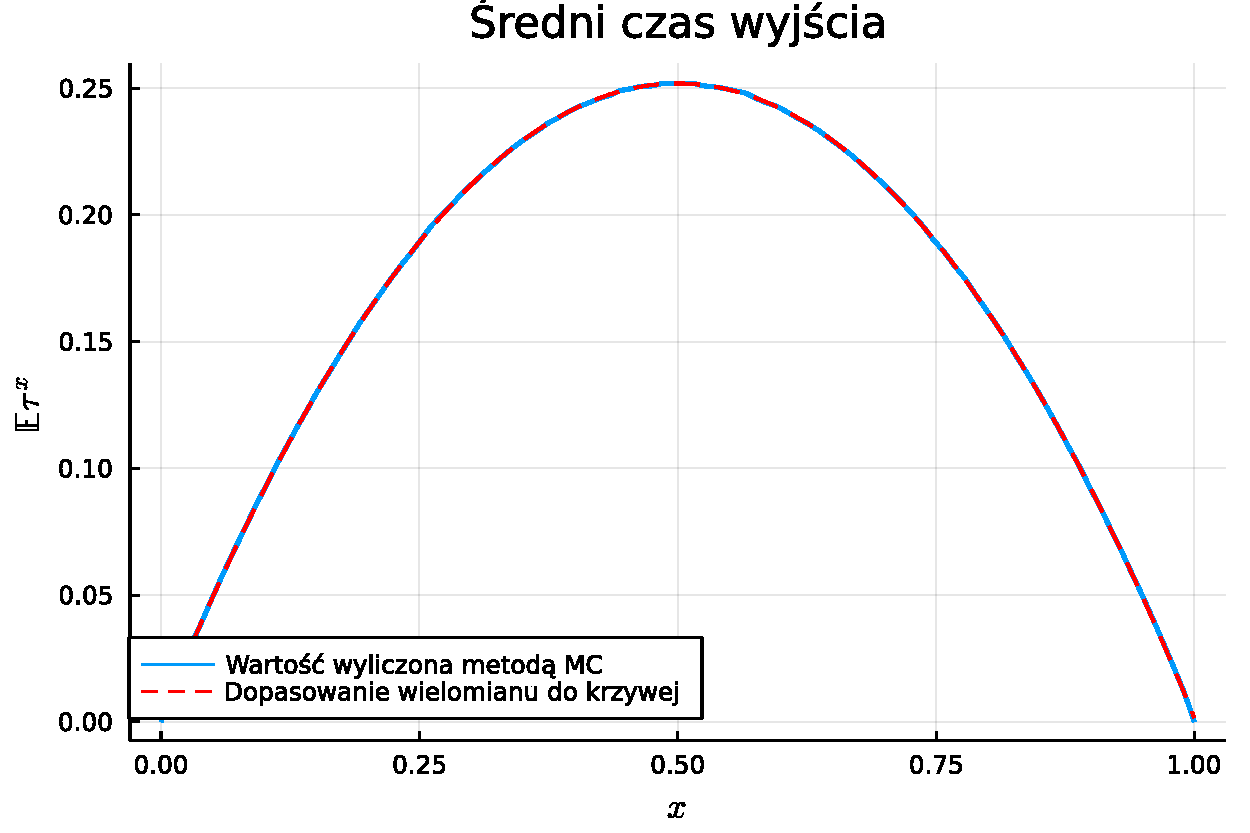
\includegraphics[width=\columnwidth]{fig/plot/expect_val.pdf}
		\caption{Oszacowanie wartości oczekiwanej czasu wyjścia w zależności od punktu początkowego}
	\end{figure}
%	\noindent Patrząc na wykres podejrzewaliśmy, że jest on wielomianem. Z pomocą pakietów matematycznych udało nam się dopasować funkcję $-1,0012y^2+1,0012y+0,0016$, która jak widzimy, dobrze przybliża otrzymaną krzywą.\\
	\noindent Kształt wykresu mógł sugerować, że funkcja $f(y)=\mathbb{E}\widetilde\tau^y$ jest wielomianem. Z pomocą pakietów matematycznych udało nam się dopasować funkcję 
	\begin{equation}\label{eq:oszac}
		f(y)=-1,0012y^2+1,0012y+0,0016,
	\end{equation}
	która jak widzimy na wykresie, dobrze przybliża otrzymaną krzywą.\vspace{1.5mm}\\
	Wartość oczekiwana czasu wyjścia dla standardowego procesu Wienera jest znana\textsuperscript{\cite{art}}
%	Znana jest dokłada wartość wyjścia dla procesu Wienera\textsuperscript{\cite{art}}
	\begin{equation*}
		\mathbb{E}\mathbb{\tau}=ab,
	\end{equation*}
	gdzie $\tau$ jest czasem wyjścia z przedziału $[-a, b]$. Stąd, uwzględniając przesunięcie początkowe naszego procesu, otrzymujemy
	\begin{equation*}
		\mathbb{E}\widetilde\tau^y=y(1-y).
	\end{equation*}
	Stosując niewielkie przybliżenie (do 2-giego miejsca po przecinku) do funkcji \eqref{eq:oszac}, otrzymujemy wartość teoretyczną. Dodatkowo, korzystając teraz z \eqref{eq:tau_przeskalowane} oraz $y=(x-a)/(b-a)$ możemy uogólnić wzór na dowolny przedział $[a, b]$, otrzymując
	\begin{equation*}
		\mathbb{E}\tau^x=(b-a)^2\frac{x-a}{b-a}\left(1-\frac{x-a}{b-a}\right)=-(x-b)(x-a)
	\end{equation*}

%	Wynik otrzymany przez nasz nie różni się bardzo od wyniku analitycznego 
	
	\subsection{Prawdopodobieństwo wyjścia przez b}
	\noindent Chcieliśmy jeszcze sprawdzić jak często wyjście nastąpi przez większy z końców przedziału, czyli%większą z wartości końców przedziału, czyli
	\begin{equation*}
		\mathbb{P}\left(B^x_{\tau^x}=b\right).
	\end{equation*}
%	Korzystając z własności udowodnionych wcześniej oraz wykorzystując, że zmienna $B^x_{\tau^x}$ ma rozkład dwupunktowy skupiona na $\{a, b\}$, możemy prosto przekształcić to prawdopodobieństwo do postaci
	Korzystając z własności udowodnionych wcześniej, przekształciliśmy powyższy wzór do postaci%możemy prosto przekształcić to prawdopodobieństwo do postaci
	\begin{equation*}
		\mathbb{P}\left(B^y_{\widetilde\tau^y}=1\right),
	\end{equation*}
	gdzie $\widetilde\tau^y$ jest czasem wyjścia procesu z przedziału $[0, 1]$. By oszacować to prawdopodobieństwo ponownie skorzystaliśmy z metody Monte Carlo. Niestety generując trajektorię procesu generujemy punkty dyskretne, sprawdzając czy w danym momencie $B^x_t\geqslant b$. Prawdopodobieństwo, że trafimy dokładnie w punkt $b$ jest zatem znikome. Ponieważ $B^x_{\tau^x}$ może przyjmować jedynie dwie wartości, $a$ oraz $b$ ($b>a$), możemy przekształcić to prawdopodobieństwo, otrzymując
	\begin{equation}\label{eq:dyskretyzaction}
		\mathbb{P}\left(B^x_{\tau^x}=b\right)=\mathbb{P}\left(B^y_{\widetilde{\tau}^y}\geqslant1\right).
	\end{equation}
	 Wykorzystując powyższy wzór, byliśmy w stanie wygenerować poniższy wykres.
	\begin{figure}[H]
		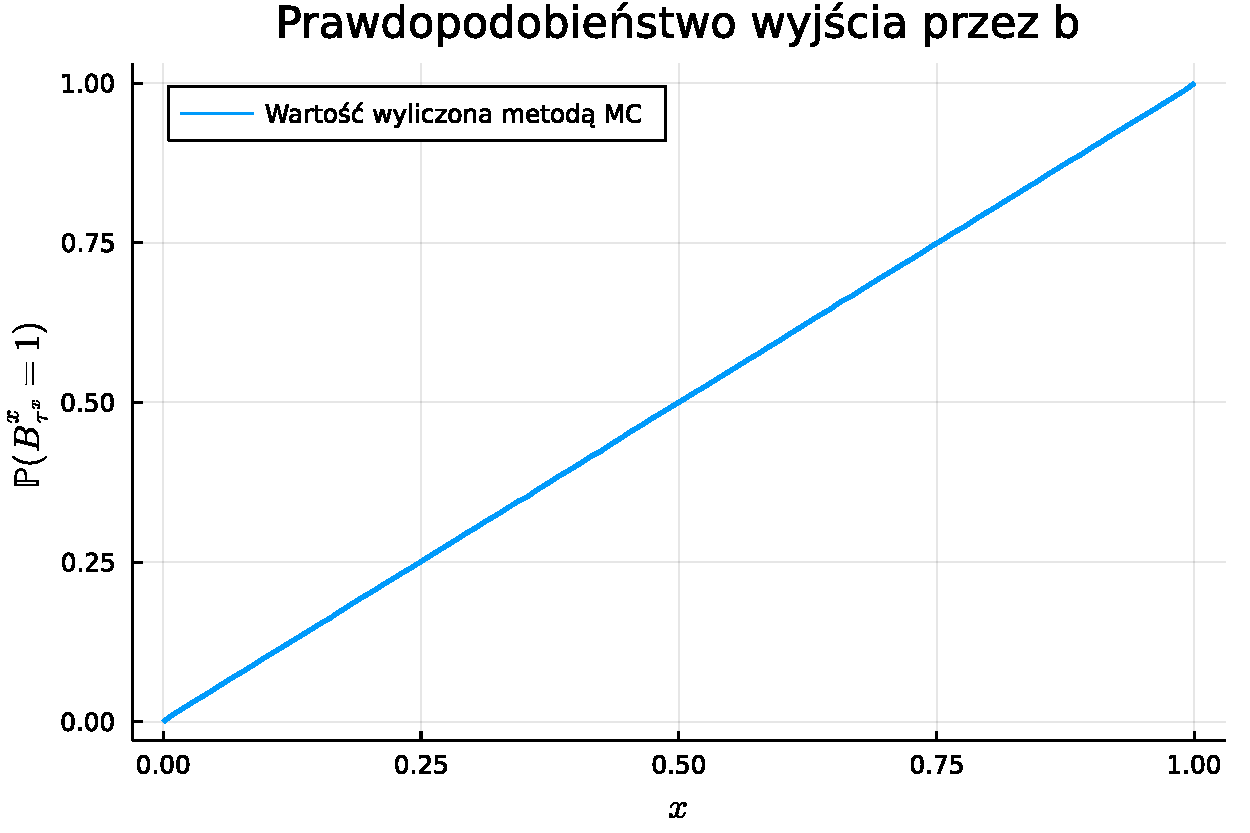
\includegraphics[width=\columnwidth]{fig/plot/prob.pdf}
		\caption{Prawdopodobieństwo wyjścia przez punkt 1.}
	\end{figure}
	\noindent Na wykresie widoczna jest zależność liniowa $\mathbb{P}\left(B^y_{\widetilde{\tau}^y}\geqslant1\right) = y$ dla $y\in[0, 1]$. Korzystając z równości \eqref{eq:dyskretyzaction} oraz $y=(x-a)/(b-a)$ , szukane prawdopodobieństwo możemy przybliżać funkcją
	\begin{equation}\label{eq:zad2_res}
		\mathbb{P}\left(B^x_{{\tau}^x}= b\right)=\frac{x-a}{b-a}.
	\end{equation}
	Podobnie jak przy wyznaczaniu wartości oczekiwanej, znany jest nam wynik analityczny\textsuperscript{\cite{art}} dla procesu Weinera startującego w 0
	\begin{equation*}
		\mathbb{P}\left(W_{\tau}=b\right)=\frac{a}{b+a},
	\end{equation*}
	gdzie $\tau$ to czas wyjścia tego procesu z przedziału $[-a, b]$. Uwzględniając przesunięcie punktu początkowego szukane przez nas prawdopodobieństwo wynosi dokładnie
	\begin{equation*}
			\mathbb{P}\left(B^x_{\tau^x}=b\right)=\mathbb{P}\left(W_{\tau}=b-x\right)=\frac{x-a}{(b-x)+(x-a)}=\frac{x-a}{b-a}.
	\end{equation*}
	Powyższy wzór pokrywa ze wzorem \eqref{eq:zad2_res} uzyskanym przy pomocy symulacji.
%	\begin{equation*}
%		\mathbb{P}\left(B^x_{\tau^x}=b\right)=\mathbb{P}\left(B^y_{\widetilde\tau^y}=1\right)=\frac{y}{1-y+y}=y,
%	\end{equation*}
%	więc wyniki naszej symulacji pokrywają się z rozwiązaniami analitycznymi.









	
	\section{Podsumowanie}
	\noindent W zadaniu 1, korzystając z różnych metod statystycznych, udało nam się dopasować model klasycznego procesu Ryzyka do danych, co potwierdziło między innymi porównanie funkcji średniej procesu ze średnią z trajektorii z danych. Następnie wykorzystaliśmy wyznaczony model do oszacowania prawdopodobieństwa ruiny. Dokonaliśmy tego korzystając z metody Monte Carlo, a w przypadku nieskończonego czasu, ogromnie przydatny okazał się wzór Pollaczka-Chinczyna. Zgodnie z intuicją okazało się, że wraz ze zwiększaniem czasu, prawdopodobieństwo ruiny rośnie, jednak nie może przekroczyć tego dla nieskończonego czasu.
	
	
	
	\section{pod budnik}
	
	
	Połączenie
	
%	Chcieliśmy oszacować średni czas wyjścia procesu Wienera z danego przedziału oraz prawdopodobieństwo wyjścia przez dany jego koniec, w zależności od punktu startowego.
	\noindent Celem drugiego zadania oszacowanie funkcje $x\mapsto\mathbb{E}\tau^x$ oraz $x\mapsto\mathbb{P}\left(B^x_{\tau^x}=b\right)$.
	Zanim do tego przystąpiliśmy pokazaliśmy, że rozpatrywany przedział mogliśmy wybrać swobodnie oraz sposób jak uogólnić otrzymane wyniki na dowolny inny. Obie funkcje oszacowaliśmy metodą Monte Carlo. W ten sposób otrzymaliśmy szukane funkcje
	\begin{equation*}
		\mathbb{E}\tau^x=-(x-b)(x-a)\quad\text{ oraz }\quad\mathbb{P}\left(B^x_{\tau^x}=b\right)=\frac{x-a}{b-a}.
	\end{equation*}
	Otrzymane wyniki bardzo dobrze odzwierciedlają wartości teoretyczne.\vspace{1.5mm}\\
	\noindent Dodatkowo podczas symulacji zauważyliśmy jak ważne jest generowanie procesu Wienera z odpowiednio mały krok czasowy. Wraz ze wzrostem wielkości kroku rósł, średni czas wyjścia procesu. By uzyskać dokładne dane generowaliśmy proces z krokiem $h=10^{-4}$.
	
	
	
	
	
	
	\newpage
	\begin{thebibliography}{1}
		\bibitem{art}
		\url{https://galton.uchicago.edu/~lalley/Courses/313/BrownianMotionCurrent.pdf}
	\end{thebibliography}


\end{document}